
\documentclass[10pt]{scrreprt} % Default font size and left-justified equations
\KOMAoptions{parskip=half}

\usepackage[top=2cm,bottom=2cm,inner=1cm,outer=1cm, a4paper]{geometry} % Page margins

\usepackage{xcolor, colortbl} % Required for specifying colors by name
\definecolor{bleu}{RGB}{0,102,204} % Define the blue color used for highlighting throughout the book
\definecolor{mygreen}{rgb}{0,0.6,0}
\definecolor{mygray}{rgb}{0.5,0.5,0.5}
\definecolor{mymauve}{rgb}{0.58,0,0.82}

\usepackage[french]{babel}  % French language
\DecimalMathComma
\usepackage[bitstream-charter]{mathdesign}

% Index
\usepackage{calc} % For simpler calculation - used for spacing the index letter headings correctly
\usepackage{makeidx} % Required to make an index
\makeindex % Tells LaTeX to create the files required for indexing

\usepackage{markdown}
%----------------------------------------------------------------------------------------
%	VARIOUS REQUIRED PACKAGES
%----------------------------------------------------------------------------------------
\usepackage{amsmath,amsfonts,amsthm} % For math equations, theorems, symbols, etc
\usepackage{esint}
\usepackage{siunitx}
\sisetup{locale = FR,inter-unit-product =\cdot}
\usepackage{titlesec} % Allows customization of titles

\usepackage{graphicx} % Required for including pictures
\usepackage{rotating}
\usepackage{wrapfig}
\usepackage{caption}
\usepackage{subcaption}
\usepackage{tabularx}

\usepackage{diagbox}

\usepackage{array}
\newcommand{\PreserveBackslash}[1]{\let\temp=\\#1\let\\=\temp}
\newcolumntype{C}[1]{>{\PreserveBackslash\centering}m{#1}}
\newcolumntype{R}[1]{>{\PreserveBackslash\raggedleft}m{#1}}
\newcolumntype{L}[1]{>{\PreserveBackslash\raggedright}m{#1}}


\graphicspath{./Pictures/} % Specifies the directory where pictures are stored
\renewcommand{\thefigure}{\arabic{section}.\arabic{figure}}
\renewcommand{\thetable}{\arabic{section}.\arabic{table}}

\usepackage{tikz} % Required for drawing custom shapes
\usetikzlibrary{trees,arrows,patterns,plotmarks, positioning}
\usepackage{forest}

\usepackage{pgfplots}
\usepackage{pgfplotstable}
\pgfplotsset{compat=1.10}
\usepgfplotslibrary{fillbetween}

\usepackage{enumitem} % Customize lists
\usepackage[f]{esvect}

\setlist{itemsep=1pt,topsep=1pt} % Reduce spacing between bullet points and numbered lists
\setitemize{label=\textbullet}

\usepackage{booktabs} % Required for nicer horizontal rules in tables

\usepackage{eso-pic} % Required for specifying an image background in the title page

\usepackage{multicol,multirow}
\usepackage{filecontents}

\usepackage{float}

%---------------
% 	 CODE
%---------------
\usepackage{minted}
\usepackage{tcolorbox}
\tcbuselibrary{listings, minted, skins}

\newfloat{lstfloat}{htbp}{lop}
\floatname{lstfloat}{Listing}
\def\lstfloatautorefname{Listing}

\tcbset{listing engine=minted}
\usemintedstyle[python]{tango}
\usemintedstyle[pycon]{tango}
\setmintedinline[python]{fontsize = \small}
\newcommand{\pyinline}[1]{\mintinline{python}{#1}}

\newtcblisting{pythonlst}{	listing only, minted language=python,
	sharp corners,
	width=10cm,
	minted options={%fontfamily=jkptt, 
		fontsize=\footnotesize, tabsize=2, breaklines, autogobble}, enhanced,frame hidden, 
	overlay unbroken and last={%
		\draw[line width=1mm, gray] (interior.north west)++(0,-0.25cm)   -- (interior.north west)-- (interior.north east)-- ++(0,-0.25cm) ;
		\draw[line width=1mm, gray] (interior.south west)++(0,0.25cm)   -- (interior.south west)-- (interior.south east)-- ++(0,0.25cm) ;}}

\newtcbinputlisting{\inputPython}[3]{listing file={#1},
	listing only, minted language=python,
	sharp corners,
	width=10cm,
	minted options={firstline=#2,lastline=#3,linenos, %fontfamily=jkptt, 
		fontsize=\footnotesize, tabsize=2, breaklines, autogobble}, enhanced,frame hidden, 
	overlay unbroken and last={%
		\draw[line width=1mm, gray] (interior.north west)++(0,-0.25cm)   -- (interior.north west)-- (interior.north east)-- ++(0,-0.25cm) ;
		\draw[line width=1mm, gray] (interior.south west)++(0,0.25cm)   -- (interior.south west)-- (interior.south east)-- ++(0,0.25cm) ;}}


\usepackage[noend]{algpseudocode}
\algrenewcommand\algorithmicwhile{\texttt{while}}
\algrenewcommand\algorithmicdo{\texttt{do}}
\algrenewcommand\algorithmicif{\texttt{if}}
\algrenewcommand\algorithmicthen{\texttt{then}}
\algrenewcommand\algorithmicelse{\texttt{else}}
\algnewcommand\Skip{\texttt{skip}}%	

%----------------------------------------------------------------------------------------
%	HYPERLINKS IN THE DOCUMENTS
%----------------------------------------------------------------------------------------

% For an unclear reason, the package should be loaded now and not later
\usepackage{hyperref}
\hypersetup{
	colorlinks,
	linkcolor={red!50!black},
	citecolor={blue!50!black},
	urlcolor={blue!80!gray}
}

%----------------------------------------------------------------------------------------
%	SECTION NUMBERING
%----------------------------------------------------------------------------------------
\setcounter{tocdepth}{3}
\setcounter{secnumdepth}{3}
\renewcommand\thesection{\arabic{section}}
\renewcommand\thesubsection{\arabic{section}.\arabic{subsection}}
\renewcommand\thesubsubsection{\arabic{section}.\arabic{subsection}.\arabic{subsubsection}}

%-------Set parskip for minipages--------
\makeatletter 
\let\org@parboxrestore\@parboxrestore 
\def\@parboxrestore{% 
  \edef\restore@parsettings{% 
    \parindent=\the\parindent\relax 
    \parskip=\the\parskip\relax 
  }% 
  \org@parboxrestore 
  \restore@parsettings 
} 
\makeatother 
 % Insert the commands.tex file which contains the majority of the structure behind the template

%equations sur plusieurs lignes, avec ou sans accolades
\newcommand\meq[1]{\begin{equation*}\begin{split}#1\end{split}\end{equation*}}
\newcommand\meqa[1]{\begin{equation*}\left\{\begin{split}#1\end{split}\right.\end{equation*}}

%Vecteurs (bases, opérateurs,...)
\newcommand\ux{\vv{u}_x}
\newcommand\uy{\vv{u}_y}
\newcommand\uz{\vv{u}_z}
\newcommand\ur{\vv{u}_r}
\newcommand\ut{\vv{u}_\theta}
\newcommand\uf{\vv{u}_\varphi}

\newcommand\ve[1]{\vv{#1}}

\newcommand\grad{\ve{\mathrm{grad}\,}}
\newcommand\dive{\mathrm{div}\,}
\newcommand\rot{\ve{\mathrm{rot}}\,}

%Opérateurs différentiels
\newcommand\dt[1]{\dfrac{\mathrm d #1}{\mathrm d t}}
\newcommand\ddt[1]{\dfrac{\mathrm d^2 #1}{\mathrm d t^2}}
\newcommand\Dt[1]{\dfrac{\mathrm D #1}{\mathrm D t}}

\newcommand\de {\mathrm d}
\newcommand\De {\mathrm D}

\newcommand\diff[2]{\dfrac{\mathrm d #1}{\mathrm d #2}}
\newcommand\pdiff[2]{\dfrac{\partial #1}{\partial #2}}

\newcommand\ddiff[2]{\dfrac{\mathrm d^2 #1}{\mathrm d #2^2}}
\newcommand\pddiff[2]{\dfrac{\partial^2 #1}{\partial #2^2}}

%unités
\newcommand\un[1]{\mathrm{\, #1}}


\title{UPSimulator}
\author{Maxence KLEIN\\ \and Véronique REYNAUD\\ \and Guillaume DESJOUIS }
\date{2020}

\begin{document}
\maketitle
\tableofcontents
\clearpage

\section{Présentation générale du projet}
Le projet \textsc{UPSimulator} a pour objectif de développer un simulateur de processeur à visée pédagogique. Celui-ci doit permettre d'appréhender la chaine conduisant d'un programme écrit dans un langage de haut niveau au détail de l'exécution à l'échelle du processeur. Pour cela, le projet doit permettre:
\begin{itemize}
	\item la production d'un code source dans un langage jouet;
	\item la compilation du code source et la production d'une version assembleur et binaire de celui-ci. Le simulateur doit permettre l'usage de différents modèles (taille des mots binaires, nombre de registre, ...);
	\item le suivi de l'exécution (registres, mémoire, pointeur, appels à l'UAL,...);
\end{itemize}

Les choix techniques retenus pour chaque fonctionnalité sont développés ci-après.

\begin{figure}[h!]
	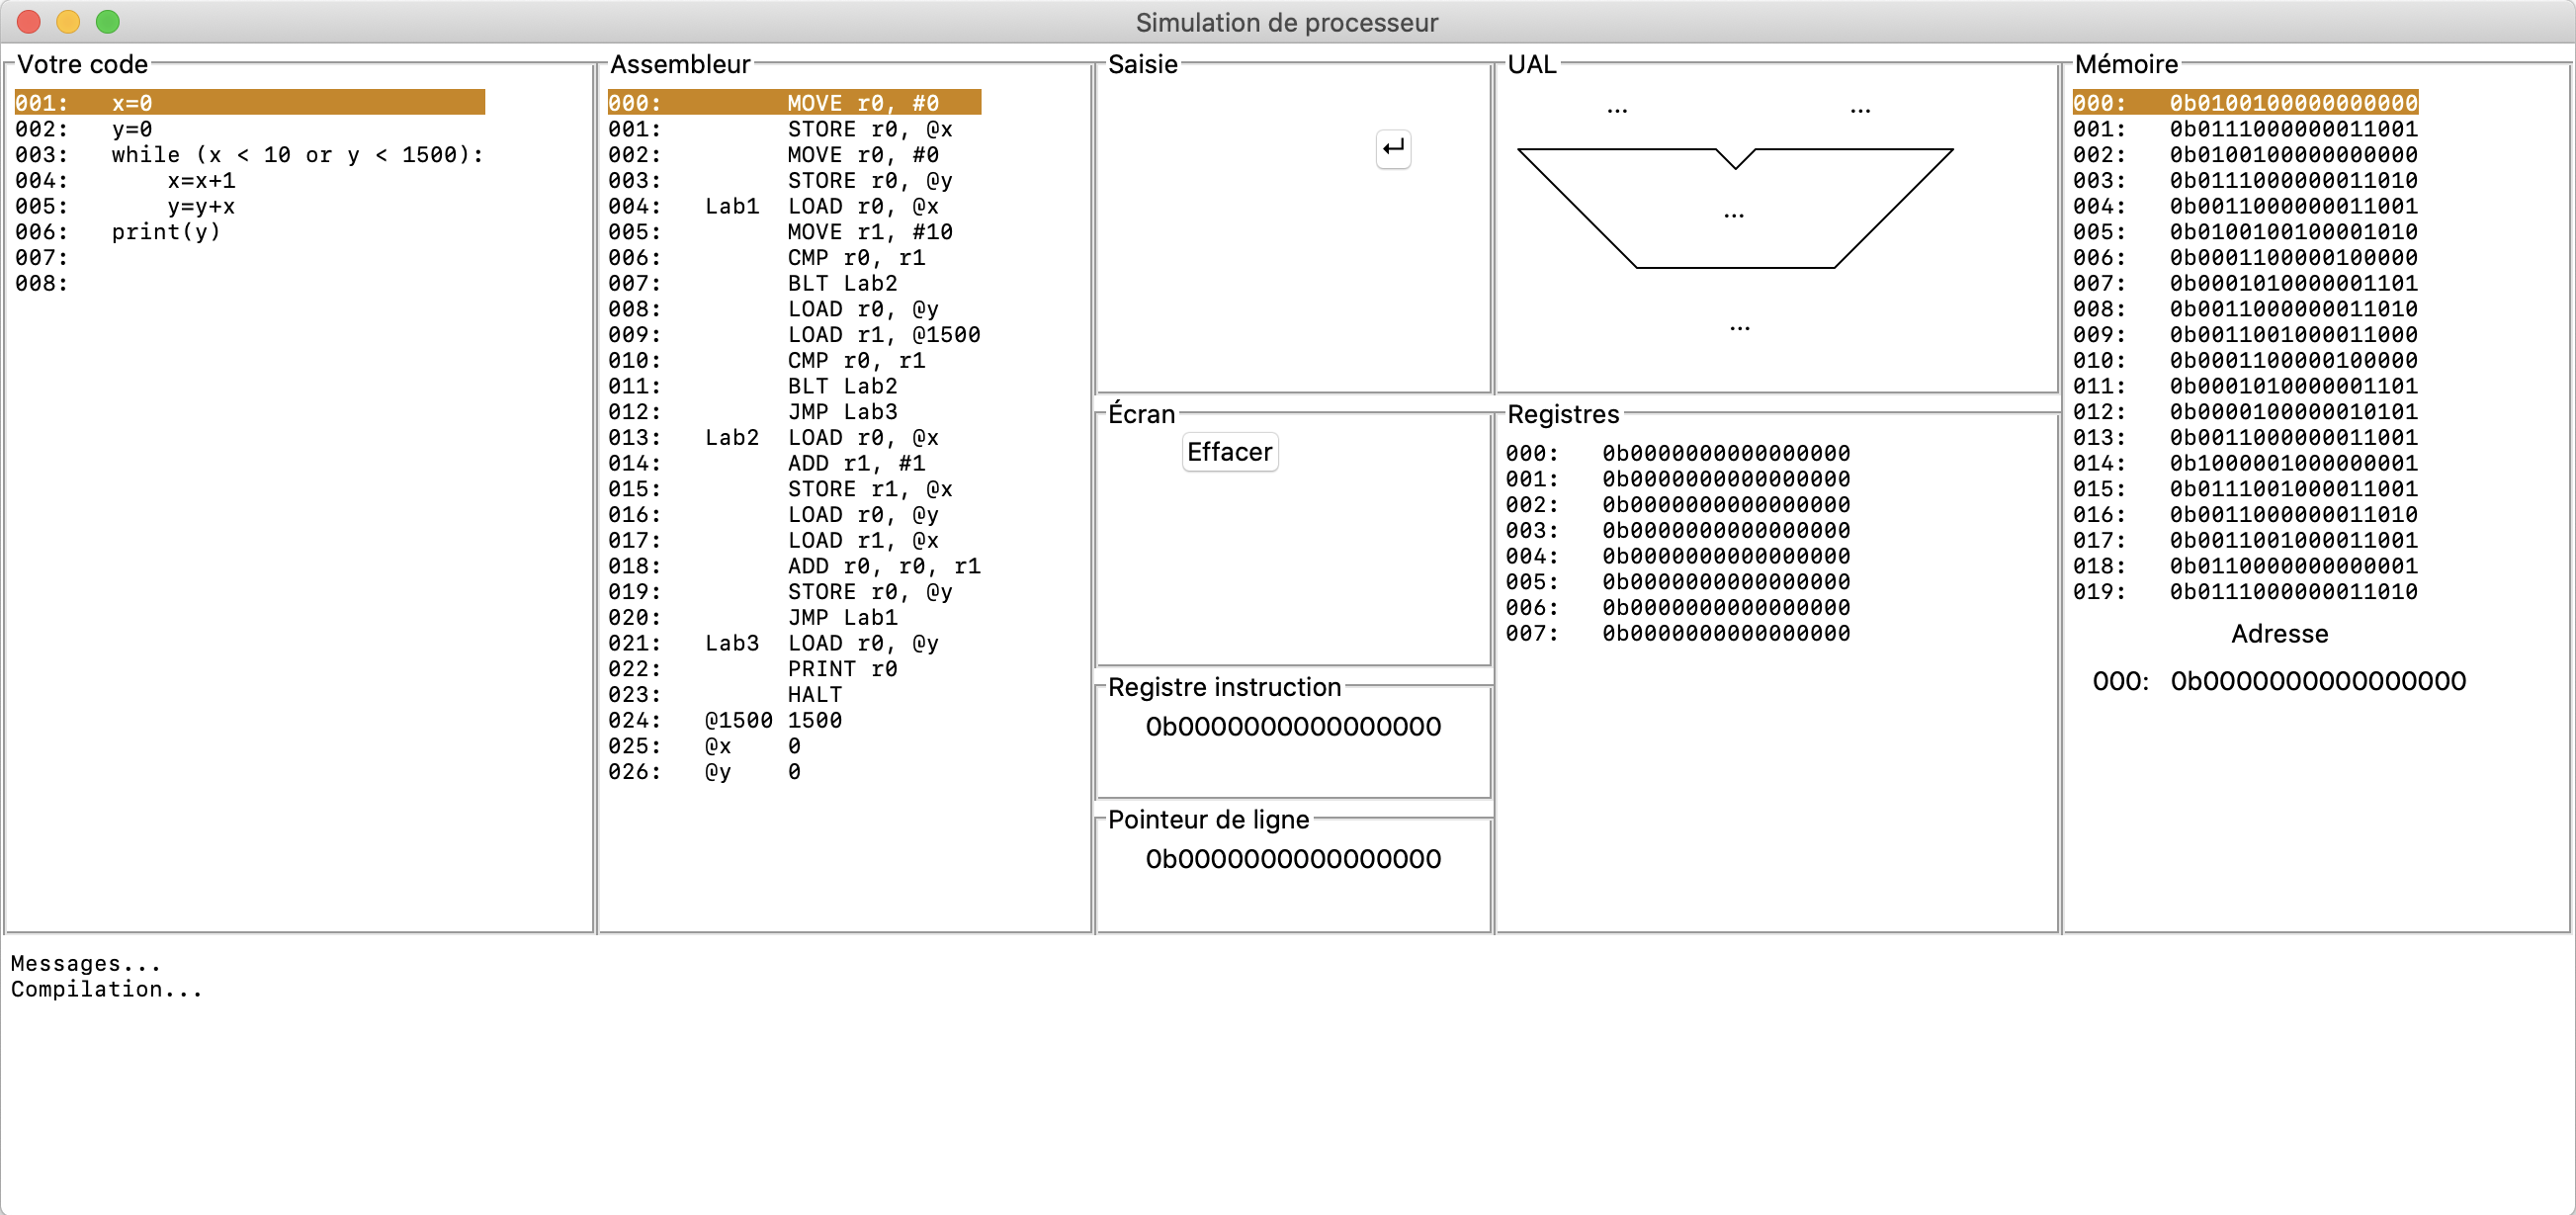
\includegraphics[width=\textwidth]{./Pictures/Header.png}
	\caption{\label{fig:gui} Interface Graphique}
\end{figure}


\clearpage
\section{Choix techniques}
\subsection{Langage jouet}

Le langage jouet doit permettre à l'utilisateur de produire un exemple de code simple reprenant les principales structures (boucles, branchements conditionnels,...)

\begin{lstfloat}[h!]
	\centering
\inputPython{example2.code}{1}{11}
\caption{Exemple de code dans le langage jouet}
\end{lstfloat}

\subsubsection{Expressions admissibles}

Les expression admissibles sont présentées dans la table  \ref{tab:expressions} ci-dessous.
\begin{table}[h!]\caption{\label{tab:expressions}Expressions admissibles}
	\centering
	\begin{tabular}{|c|c|c|}
	\hline
	\multicolumn{2}{|c|}{Variable}   &            \pyinline{x}            \\ \hline
	\multicolumn{2}{|c|}{Entier}     &            \pyinline{n}            \\ \hline
	              &      Somme       &         \pyinline{e1 + e2}         \\ \cline{2-3}
	              &    Différence    &         \pyinline{e1 - e2}         \\ \cline{2-3}
	 Opérations   &     Produit      &         \pyinline{e1 * e2}         \\ \cline{2-3}
	arithmétiques & Division entière &         \pyinline{e1 / e2}         \\ \cline{2-3}
	              &      Reste       & \pyinline{e1 % e2
	              } \\ \cline{2-3}
	              &      Opposé      &           \pyinline{-e1}           \\ \hline
\end{tabular}
\hspace{3cm}
\begin{tabular}{|c|c|c|}
	\hline
	\multicolumn{3}{|c|}{Opérations logiques}                                         \\ \hline
	\multirow{10}{*}{Binaires} &           Egalité           &  \pyinline{e1 == e2}   \\ \cline{2-3}
	                           &         Différence          &  \pyinline{e1 != e2}   \\ \cline{2-3}
	                           & \multirow{4}{*}{Inégalités} &   \pyinline{e1 < e2}   \\ \cline{3-3}
	                           &                             &   \pyinline{e1 > e2}   \\ \cline{3-3}
	                           &                             &  \pyinline{e1 <= e2}   \\ \cline{3-3}
	                           &                             &  \pyinline{e1 >= e2}   \\ \cline{2-3}
	                           &     \multirow{2}{*}{Et}     &  \pyinline{e1 and e2}  \\ \cline{3-3}
	                           &                             &  \pyinline{e1 \& e2}   \\ \cline{2-3}
	                           &     \multirow{2}{*}{Ou}     &  \pyinline{e1 or e2}   \\ \cline{3-3}
	                           &                             & \pyinline{e1     | e2} \\ \hline
	 \multirow{2}{*}{Unaire}   &      inverse bit à bit      &     \pyinline{~e1}     \\ \cline{2-3}
	                           &      négation logique       &   \pyinline{not e1}    \\ \hline
\end{tabular}
\end{table}
%
\subsubsection{Liste de commandes admissibles}

\begin{minipage}[c]{0.38\textwidth}
	\begin{minted}[frame = single, label={Affectation}]{python}
x=e
\end{minted}
\end{minipage}
\hspace{1cm}
\begin{minipage}[c]{0.38\textwidth}
	avec \pyinline{e} une expression logique ou arithmétique.
\end{minipage}
\vspace{0.5cm}

\begin{minipage}[c]{0.38\textwidth}
\begin{minted}[frame = single, label={Branchement conditionnel}]{python}
if e :
	c1
elif e2: 
	c2
else:
	c3
\end{minted}
\end{minipage}
\hspace{1cm}
\begin{minipage}[c]{0.38\textwidth}
	avec \pyinline{e1} et \pyinline{e2} des expressions et \pyinline{c1}, \pyinline{c2} et \pyinline{c3} des commandes.
	
	Les branchement \pyinline{else} et \pyinline{elif} sont optionnels.
\end{minipage}
\vspace{0.5cm}

\begin{minipage}[c]{0.38\textwidth}
\begin{minted}[frame = single, label={Boucle}]{python}
while e :
	c1
\end{minted}
\end{minipage}
\hspace{1cm}
\begin{minipage}[c]{0.38\textwidth}
	avec \pyinline{e} une expression et \pyinline{c} une commande.	
\end{minipage}
\vspace{0.5cm}

\begin{minipage}[c]{0.38\textwidth}
\begin{minted}[frame = single, label={Lecture clavier}]{python}
input()
\end{minted}
\end{minipage}
\vspace{0.5cm}

\begin{minipage}[c]{0.38\textwidth}
\begin{minted}[frame = single, label={Ecriture sur la sortie courante}]{python}
print(v)
\end{minted}
\end{minipage}
\hfill
\begin{minipage}[c]{0.38\textwidth}
	avec \pyinline{e} une expression	
\end{minipage}

\subsubsection{Indentations}
Le code est indenté comme en python afin de détecter les blocs:
\begin{itemize}
	\item L'indentation n'augmente qu'après un \pyinline{:} lié à une structure \pyinline{if} ou \pyinline{while}
	\item L'indentation ne peut diminuer que atteindre un niveau précédemment atteint.
\end{itemize}

\subsubsection{Commentaires}
Les commentaires sont repérés par le caractère \pyinline{#} .

\begin{lstfloat}
	\begin{center}
	\begin{pythonlst}
aaaaaaaaaa:
	aaaaaaaaaa
	aaaaaaaaaa
		aaaaaaaaaa # pas valable il manque : avant
		aaaaaaaaaa
	aaaaaaaaaa
aaaaaaaaaa
aaaaaaaaaa:
			aaaaaaaaaa
	aaaaaaaaaa # pas valable. Ce niveau a été atteint avant mais pas dans le même bloc
aaaaaaaaaa
\end{pythonlst}
\caption{Langage jouet - Commentaires et indentations}
\end{center}
\end{lstfloat}





\clearpage

\subsection{\label{sec:processeur}Modèle de processeur}

\subsubsection{ProcessorEngine}
Le simulateur doit offrir une certaine modularité afin de permettre d'apprécier l'incidence des choix de conception sur le code assembleur et sur l'exécution. 

Les propriétés du processeur sont gérées par la classe \pyinline{ProcessorEngine}

On pourra donc définir le modèle de processeur retenu à l'aide d'un dictionnaire qui prend pour clés:
\begin{itemize}
	\item le nom du modèle associé: \pyinline{'name': str};
	\item la taille des registres: \pyinline{'register_bits': int};
	\item la taille des mots: \pyinline{'data_bits': int};
	\item la capacité ou non de réorienter la sortie de l'UAL vers un registre quelconque: \pyinline{'free_ual_output':bool}. Si \pyinline{False}, la sortie de l'UAL sera systématique le registre 0. Il convient alors de libérer celui-ci; 
	\item la liste des commandes pouvant accepter directement des littéraux \pyinline{'litteralCommands':Dict[str,Commands]};
	\item la liste des commandes admissibles \pyinline{'commands':Dict[str,Commands]}.
\end{itemize}

Chaque \pyinline{Command} correspond à un dictionnaire qui prends pour clés:
\begin{itemize}
	\item un code binaire \pyinline{'opcode': str,}. Le choix des \pyinline{opcode} est fait de telle sorte que la taille des mots soit op
	\item une commande assembleur \pyinline{'asm': str},
	\item la taille du littéral associé	\pyinline{'litteral_bits': int}
\end{itemize}

Deux modèles sont implémentés par défaut dans le simulateur.

\begin{minipage}[t]{0.48\textwidth}
	\captionof{table}{Processeur 16 bits}
\begin{minipage}[t]{0.5\textwidth}
	\vspace{0cm}
	\centering
		\begin{tabular}{l|>{\ttfamily\footnotesize}l}
		\pyinline{register_bits}&	3\\ \hline
		\pyinline{free_ual_output}&	True
\\\hline
		\pyinline{data_bits}&	16\\
		\end{tabular}
	
	\vspace{1cm}
	
	\begin{tabular}{>{\ttfamily\footnotesize}c|>{\ttfamily\footnotesize}c|>{\ttfamily\footnotesize}c}
		\multicolumn{3}{c}{\pyinline{litteralCommands}}\\\hline\hline
		Nom	& OPCODE & ASM\\\hline
		neg                & 010110 & NEG  \\
		move               & 01001  & MOVE \\
		+                  & 1000  & ADD  \\
		-                  & 1001  & SUB  \\
		*                  & 1010  & MULT \\
		/                  & 1011  & DIV  \\
		\%                 & 1100  & MOD  \\
		\&                 & 1101  & AND  \\
		|                  & 1110  & OR   \\
		\textasciicircum{} & 1111  & XOR  \\
		$\sim$             & 010111 & NOT 
	\end{tabular}
\end{minipage}
\begin{minipage}[t]{0.5\textwidth}
	\vspace{0cm}	
	\centering
		\begin{tabular}{>{\ttfamily\footnotesize}c|>{\ttfamily\footnotesize}c|>{\ttfamily\footnotesize}c}
		\multicolumn{3}{c}{\pyinline{Commands}}\\\hline\hline
		Nom	& OPCODE & ASM\\\hline
halt               & 00000      & HALT  \\
goto               & 000001      & JMP   \\
!=                 & 0001000   & BNE   \\
==                 & 0001001   & BEQ   \\
\textless{}        & 0001010   & BLT   \\
\textgreater{}     & 0001011   & BGT   \\
cmp                & 00011     & CMP   \\
print              & 00100    & PRINT \\
input              & 00101    & INPUT \\
load               & 0011     & LOAD  \\
move               & 01000   & MOVE  \\
neg                & 010100  & NEG   \\
$\sim$             & 010101  & NOT   \\
+                  & 0110000 & ADD   \\
-                  & 0110001 & SUB   \\
*                  & 0110010 & MULT  \\
/                  & 0110011 & DIV   \\
\%                 & 0110100 & MOD   \\
\&                 & 0110101 & AND   \\
|                  & 0110110 & OR    \\
\textasciicircum{} & 0110111 & XOR   \\
store              & 0111    & STORE
\end{tabular}
\end{minipage}
\end{minipage}
\hfill
\begin{minipage}[t]{0.48\textwidth}
	\captionof{table}{Processeur 12 bits}
	\begin{minipage}[t]{0.5\textwidth}
		\vspace{0cm}
		\centering
		\begin{tabular}{l|>{\ttfamily\footnotesize}l}
			\pyinline{register_bits}&	2\\ \hline
			\pyinline{free_ual_output}&	False
\\\hline
			\pyinline{data_bits}&	12\\
		\end{tabular}
		
		\vspace{1cm}
		
		\begin{tabular}{>{\ttfamily\footnotesize}c|>{\ttfamily\footnotesize}c|>{\ttfamily\footnotesize}c}
			\multicolumn{3}{c}{\pyinline{litteralCommands}}\\\hline\hline
			Nom	& OPCODE & ASM\\\hline
			\multicolumn{3}{c}{\pyinline{NONE}}\\\hline\hline
		\end{tabular}
	\end{minipage}
	\begin{minipage}[t]{0.5\textwidth}
		\vspace{0cm}
		\centering
		\begin{tabular}{>{\ttfamily\footnotesize}c|>{\ttfamily\footnotesize}c|>{\ttfamily\footnotesize}c}
			\multicolumn{3}{c}{\pyinline{Commands}}\\\hline\hline
			Nom	& OPCODE & ASM\\\hline
			halt               & 0000       & HALT  \\
			goto               & 0001        & JMP   \\
			==                 & 0010       & BEQ   \\
			\textless{}        & 0011       & BLT   \\
			cmp                & 11110101 & CMP   \\
			print              & 0100      & PRINT \\
			input              & 0101      & INPUT \\
			load               & 100      & LOAD  \\
			move               & 11110110 & MOVE  \\
			$\sim$             & 11110111 & NOT   \\
			+                  & 11111000 & ADD   \\
			-                  & 11111001 & SUB   \\
			*                  & 11111010 & MULT  \\
			/                  & 11111011 & DIV   \\
			\%                 & 11111100 & MOD   \\
			\&                 & 11111101 & AND   \\
			|                  & 11111110 & OR    \\
			\textasciicircum{} & 11111111 & XOR   \\
			store              & 101      & STORE
		\end{tabular}
	\end{minipage}
\end{minipage}

La classe \pyinline{ProcessorEngine} a la responsabilité entre autre d'assurer que le modèle de processeur soit consistant, d'assurer la conversion entre code assembleur et code binaire.
\begin{sidewaysfigure}
	\centering
		
\tikzset{
	every leaf node/.style={draw=black, rectangle, align=center},
	every tree node/.style={font=\tiny},
	tt/.style={font=\ttfamily},
}
\forestset{tikzQtree/.style={for tree={l sep=3em, anchor=center, if n children=0{
				node options=every leaf node/.try}{node options=every tree node/.try}}}}
	\scriptsize
	\begin{forest}
		tikzQtree
[	,
	[ 0,
		[ 00,
			[ 000, 
				[ 0000
					[00000[\texttt{HALT}]],[00001[\texttt{JUMP}]]
				],
				[ 0001,
					[ 00010,
						[ 000100,
							[0001000[\texttt{BNE}]], [0001001[\texttt{BEQ}]]
						],
						[ 000100,
							[0001010[\texttt{BLT}]], [0001011[\texttt{BGT}]]
						]
					],
					[00011[\texttt{CMP}]]
				]
			],
			[ 001,
				[ 0010,
					[00100[\texttt{PRINT}]], [00101[\texttt{INPUT}]]
				],
				[0011[\texttt{LOAD}]]
			]
		],
		[ 01,
			[ 010,
				[ 0100,
					[01000[\texttt{MOVE}]], [01001[\texttt{MOVE}]],
				],
				[ 0101,
					[ 01010,
						[010100[\texttt{NEG}]], [010101[\texttt{NOT}]]
					],
					[ 01011,
					[010110[\texttt{NEG}]], [010111[\texttt{NOT}]]
					]
				]
			],
			[011
				[0110,
					[01100,
						[011000,
							[0110000[\texttt{ADD}]], [0110001[\texttt{SUB}]]
						],
						[011001,
							[0110010[\texttt{MULT}]], [0110011[\texttt{DIV}]]
						]
					],
					[01101,
						[011010,
							[0110100[\texttt{MOD}]], [0110101[\texttt{AND}]]
						],
						[011011,
							[0110110[\texttt{OR}]], [0110111[\texttt{XOR}]]
						]
					],
				],
				[0111[\texttt{STORE}]]
			]
		]
	], 
	[1,
		[10,
			[100,
				[1000[\texttt{ADD}]], [1001[\texttt{SUB}]]
			],
			[101,
				[1010[\texttt{MULT}]], [1011[\texttt{DIV}]]
			]
		],
		[11,
			[110,
				[1100[\texttt{MOD}]], [1101[\texttt{AND}]]
			],
			[111,
				[1110[\texttt{OR}]], [1111[\texttt{XOR}]]
			]
		]
	]	
]
\end{forest}
		\caption{Langage 16 bits - OPCODE et ASM}
\end{sidewaysfigure}

\begin{sidewaysfigure}
	\centering
	
\tikzset{
	every leaf node/.style={draw=black, rectangle, align=center},
	every tree node/.style={font=\tiny},
	tt/.style={font=\ttfamily},
}
\forestset{tikzQtree/.style={for tree={l sep=3em, anchor=center, if n children=0{
				node options=every leaf node/.try}{node options=every tree node/.try}}}}
	\scriptsize
	\begin{forest}
		tikzQtree
[	,
	[ 0,
		[00,
			[000,
				[0000[HALT]],
				[0001[JMP]]
			],
			[001,
				[0010[BEQ]],
				[0011[BLT]]
			]
		],
		[01,
			[010,
				[0100[PRINT]],
				[0101[INPUT]]
			]
		]
	], 
	[1,
		[10,
			[100[LOAD]],
			[101[STORE]]
		],
		[11,
			[111,
				[1111,
					[11110,
						[111101,
							[1111010,
								[11110101[CMP]]
							],
							[1111011,
								[11110110[MOVE]],
								[11110111[NOT]]
							]
						]
					],
					[11111,
						[111110,
							[1111100,
								[11111000[ADD]],
								[11111001[SUB]]
							],
							[1111101,
								[11111010[MULT]],
								[11111011[DIV]]
							]
						],
						[111111,
							[1111110,
								[111111100[MOD]],
								[111111101[AND]]
							],
							[1111111,
								[111111110[OR]],
								[111111111[XOR]]
							]
						]
					]
				]
			]
		]
	]	
]
\end{forest}
	\caption{Langage 12 bits - OPCODE et ASM}
\end{sidewaysfigure}

\clearpage
\subsubsection{Executeur}

Lors de l'exécution, le processeur modèle est représenté par un objet de classe \pyinline{Executeur} (figure \ref{fig:class_Executeur}). Les différents paramètres (taille des registres, taille mémoire, fonctionnement UAL) sont définis par la classe \pyinline{ProcessorEngine} associée. Afin de permettre le suivi de l'exécution, l'\pyinline{Executeur} implémente entre autre:
\begin{itemize}
	\item 2 bus de données: \pyinline{_DATA_BUS} et \pyinline{_DATA_BUS_2};
	\item une mémoire: \pyinline{_MEMORY}
	\item un registre adresse mémoire \pyinline{_MEMORY_ADDRESS} et un registre instruction \pyinline{_INSTRUCTION_REGISTER}
	\item un pointeur de ligne \pyinline{_LINE_POINTER}
	\item une sortie affichage \pyinline{_PRINT}
	\item un buffer \pyinline{_BUFFER}
	\item une UAL \pyinline{_UAL}
\end{itemize}



Chaque composant est modélisé par une instance d'une classe dédiée ( \pyinline{ScreenComponent}, \pyinline{UalComponent}, \pyinline{RegisterGroup}, etc...) implémentant les méthodes associées au comportement de chaque composant physique, par exemple pour l'UAL:
\begin{itemize}
	\item définir l'opération à venir: \pyinline{setOperation()};
	\item mémoriser le premier opérande:\pyinline{writeFirstOperand()};
	\item mémoriser le second opérande: \pyinline{writeSecondOperand()};
	\item exécuter le calcul: \pyinline{execCalc()};
	\item lire le résultat: \pyinline{read()};
\end{itemize}


\begin{figure}[h!]
	\centering
	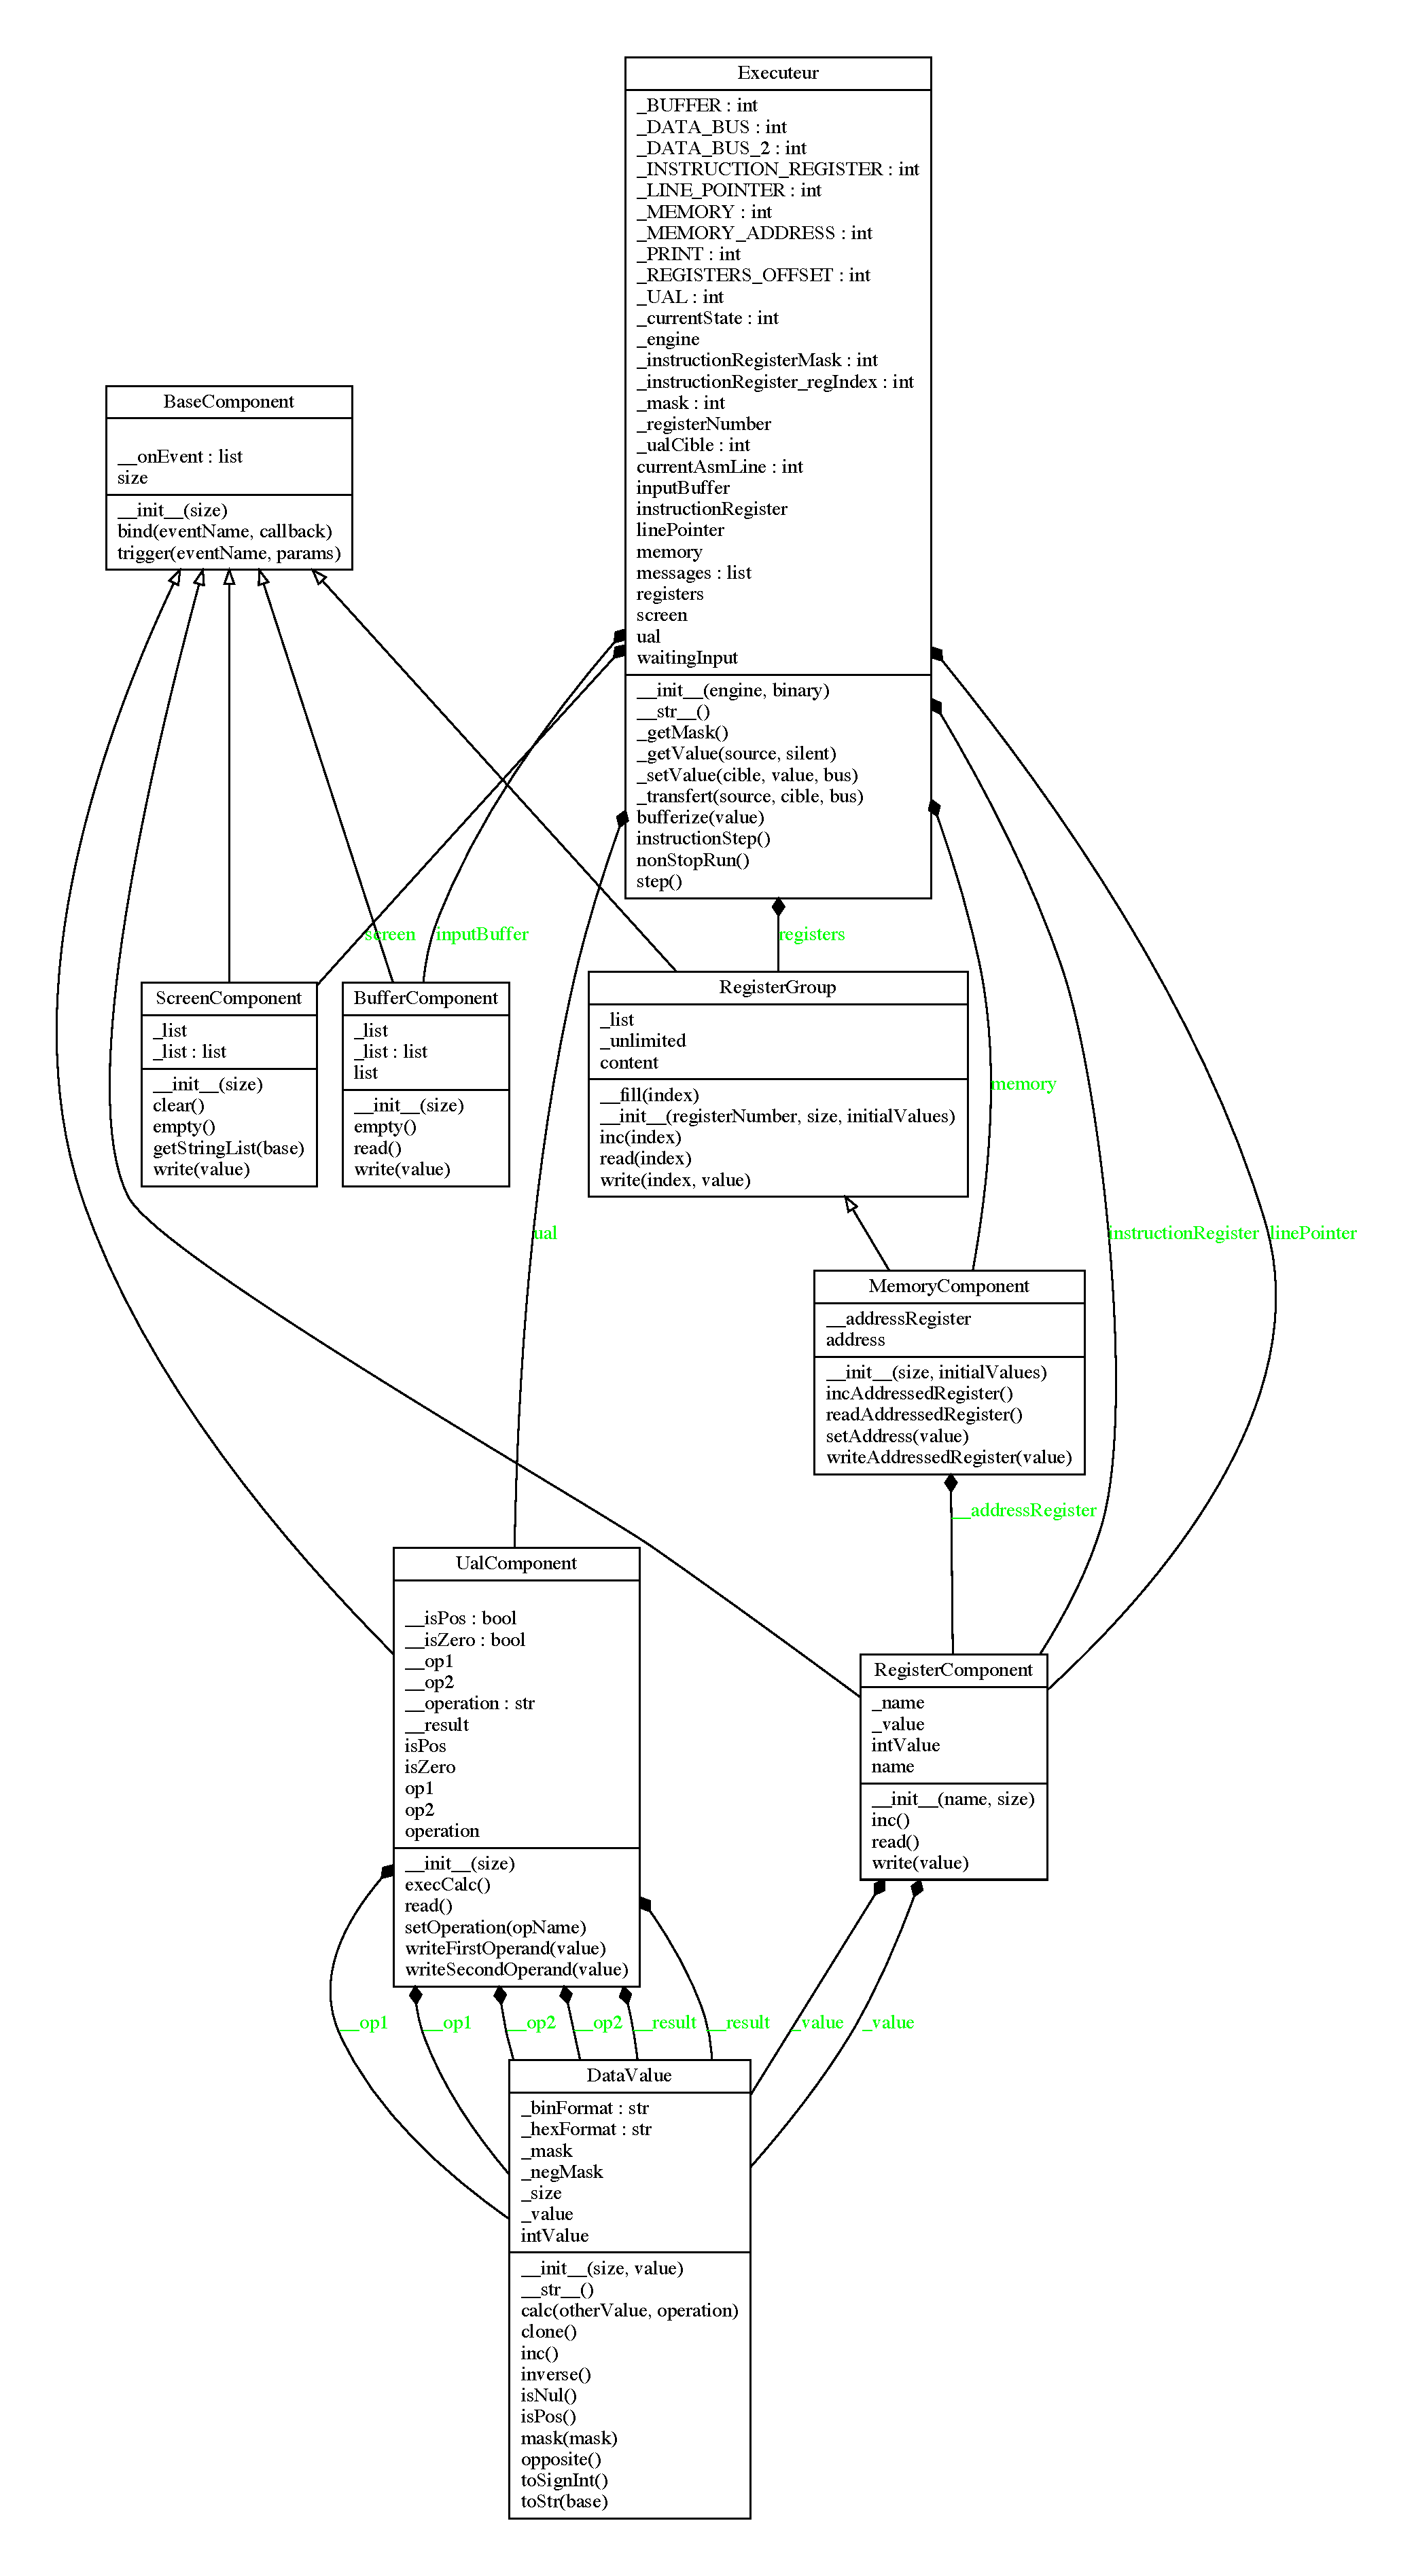
\includegraphics[height = 0.85\textheight]{./Pictures/Executeur.pdf}
	\caption{\label{fig:class_Executeur} Diagramme de classe - Executeur}
\end{figure} 

\clearpage

\subsection{\label{sec:Parsing}Parsing}


\begin{minipage}[t]{0.7\textwidth}
	Une étape d'analyse du code (parsing) est nécessaire en amont de la production du code assembleur. Cette étape a pour objet:
\begin{itemize}
	\item d'assurer que la syntaxe du langage jouet est respectée
	\item de permettre la construction d'un arbre représentant les différentes structures du code source afin de pouvoir produire le code assembleur et le binaire associé
\end{itemize}
\end{minipage}
\hfill
\begin{minipage}[t]{0.3\textwidth}
	\vspace{-1.5cm}
	\centering
	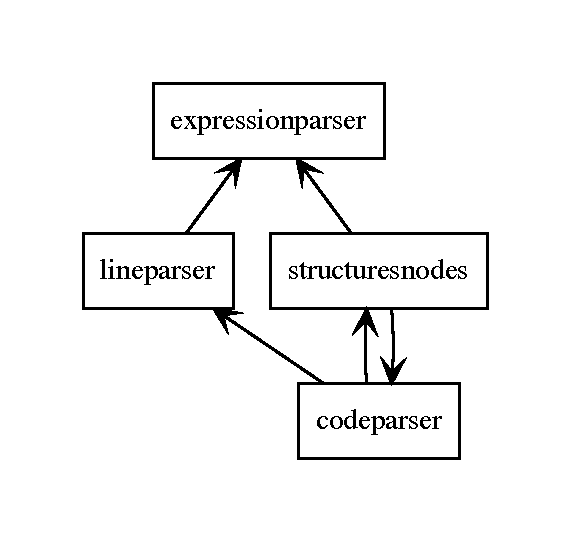
\includegraphics[scale=0.7]{./Pictures/parser.pdf}
	\captionof{figure}{}
\end{minipage}

\begin{figure}[h!]
	\centering
	\begin{tikzpicture}
	\node (ifelif) at (0,0) {
		\begin{minipage}{6cm}
		\inputminted[frame = single]{python}{example.code}
		\end{minipage}
	};
	
	
	\node[right = 4cm of ifelif.east] (ifelseif) {
\begin{minipage}{7.5cm}
\begin{minted}[frame = single]{text}
[<structuresnodes.AffectationNode >,
<structuresnodes.AffectationNode >,
<structuresnodes.WhileNode>,
<structuresnodes.PrintNode>]
\end{minted}
\end{minipage}
	};
	
	\draw[->] (ifelif.east) -- (ifelseif) node[midway, above] {\pyinline{CodeParser}};
	\end{tikzpicture}
	\caption{Exemple simpliste de parse}
\end{figure}


\subsubsection{Classe CodeParser}

L'analyse du code est gérée par un objet de la classe \pyinline{CodeParser} dont le constructeur prend en argument:
\begin{itemize}
	\item soit un nom de fichier \pyinline{filename = file}
	\item soit une chaine de caractère contenant un fragment de code \pyinline{code = fragment}
\end{itemize}

Un objet de type \pyinline{CodeParser} a pour attributs:
\begin{itemize}
	\item \pyinline{__listingCode}: une liste d'objets de type \pyinline{LineParser}
	\item \pyinline{__structuredListeNode} un arbre d'objets de type StructureNode contenant le code interprété
\end{itemize}

Lorsque le code est donné sous forme de fichier, la méthode \pyinline{__parseFile} permet de récupérer la chaîne de caractères correspondante.

La méthode \pyinline{parseCode} construit une instance de la classe \pyinline{LineParser} pour chaque ligne de code source. Si la ligne n'est pas vide, les caractéristiques de celles-ci sont ajoutées à la liste \pyinline{__listingCode}.

Une analyse syntaxique succincte est réalisée avec l'appel successif aux méthodes:
\begin{itemize}
	\item  \pyinline{__manageElif}: réécriture des branchements \pyinline{elif}).
	\begin{center}

\begin{tikzpicture}
\node (ifelif) at (0,0) {
\begin{minipage}{3cm}
\begin{minted}[frame = single]{python}
if e1 :
	c1
elif e2 :
	c2
else c3
\end{minted}
\end{minipage}
};


\node[right = 5cm of ifelif.east] (ifelseif) {
\begin{minipage}{5cm}
\begin{minted}[frame = single]{python}
if e1 :
	c1
else :
	if e2 :
		c2
	else :
		c3
\end{minted}
\end{minipage}
};

\draw[->] (ifelif.east) -- (ifelseif) node[midway, above] {\pyinline{__manageElif}};
\end{tikzpicture}
		
	\end{center}
	\item \pyinline{__blocControl}: test de la syntaxe des structures de contrôle et de l'indentation associée.
\end{itemize}


Finalement, la construction de l'arbre \pyinline{__structuredListeNode} nécessite l'appel des méthodes:
\begin{itemize}
	\item \pyinline{__buildFinalNodeList()}: construit les n\oe uds (instances de classe \pyinline{structuresnodes}) et l'arborescence correspondante à partir des caractéristiques \pyinline{__listingCode}. Les blocs d'instructions sont ajoutés à \pyinline{__structuredListeNode}.
	
	\item \pyinline{__structureList}: Parcours du listing \pyinline{__listingCode} pour ranger les enfants et leur associer le bon niveau d'indentation
\end{itemize} 


L'arborescence des n\oe uds \pyinline{__listingCode} peut-être affichée à l'aide des méthodes des \pyinline{__str__} et \pyinline{__recursiveStringifyLine}.

L'accès à la liste de n\oe uds \pyinline{__structureList} est possible à l'aide de l'accesseur \pyinline{getFinalParse}.

\subsubsection{Classe LineParser}

La classe \pyinline{LineParser} permet de renvoyer les caractéristiques d'une ligne de code sous forme d'un dictionnaire contenant numéro de ligne, niveau d'indentation, caractère vide ou non, motif identifié (if,....), condition, expression ou variable le cas échéant.

Pour une ligne de code donnée elle doit:
\begin{itemize}
	\item Nettoyer le code des commentaires et espaces terminaux: \pyinline{__suppCommentsAndEndSpaces}
	\item Déterminer le niveau d'indentation: \pyinline{__countIndentation}
	\item Pour les lignes non vides, identifier le motif: \pyinline{__identificationMotif}
\end{itemize}

Lorsque le motif correspond à un branchement conditionnel \pyinline{if e} ou une boucle \pyinline{while e} l'identification du motif \pyinline{__identificationMotif} nécessite de tester que \pyinline{e} est une expression valide. L'expression correspondante est construite par une instance de la classe \pyinline{ExpressionParser}.


\subsubsection{Classe ExpressionParser}

Les objets de la classe \pyinline{ExpressionParser}  permettent l'interprétation d'une chaine de caractère afin de renvoyer un objet de type expression, c'est à dire un arbre dont chaque n\oe ud représente un opérateur binaire, un opérateur unaire, une variable ou un littéral.

Pour cela la chaine de caractère représentant l'expression est convertie en une liste de Tokens (\pyinline{__buildTokensList(cls, expression:str) }) représentant chaque type admissible dans la chaine de caractère

La classe doit permettre de vérifier la syntaxe de l'expression 


\subsection{\label{sec:ParsedCode}Structure de donnée du code analysé}
A l'issue de la phase d'analyse, le code est disponible sous la forme d'une liste de \pyinline{StructureNode} (figure \ref{fig:parse_exemple}). C'est à partir de cette liste que sera produit le code assembleur et le code binaire associé.

L'ensemble des classes décrites ci-dessous font l'objet d'un transtypage permettant d'afficher celles-ci sous la forme d'une chaîne de caractères. 

\subsubsection{Classe StructureNode}

\begin{figure}[h!]
	\centering
	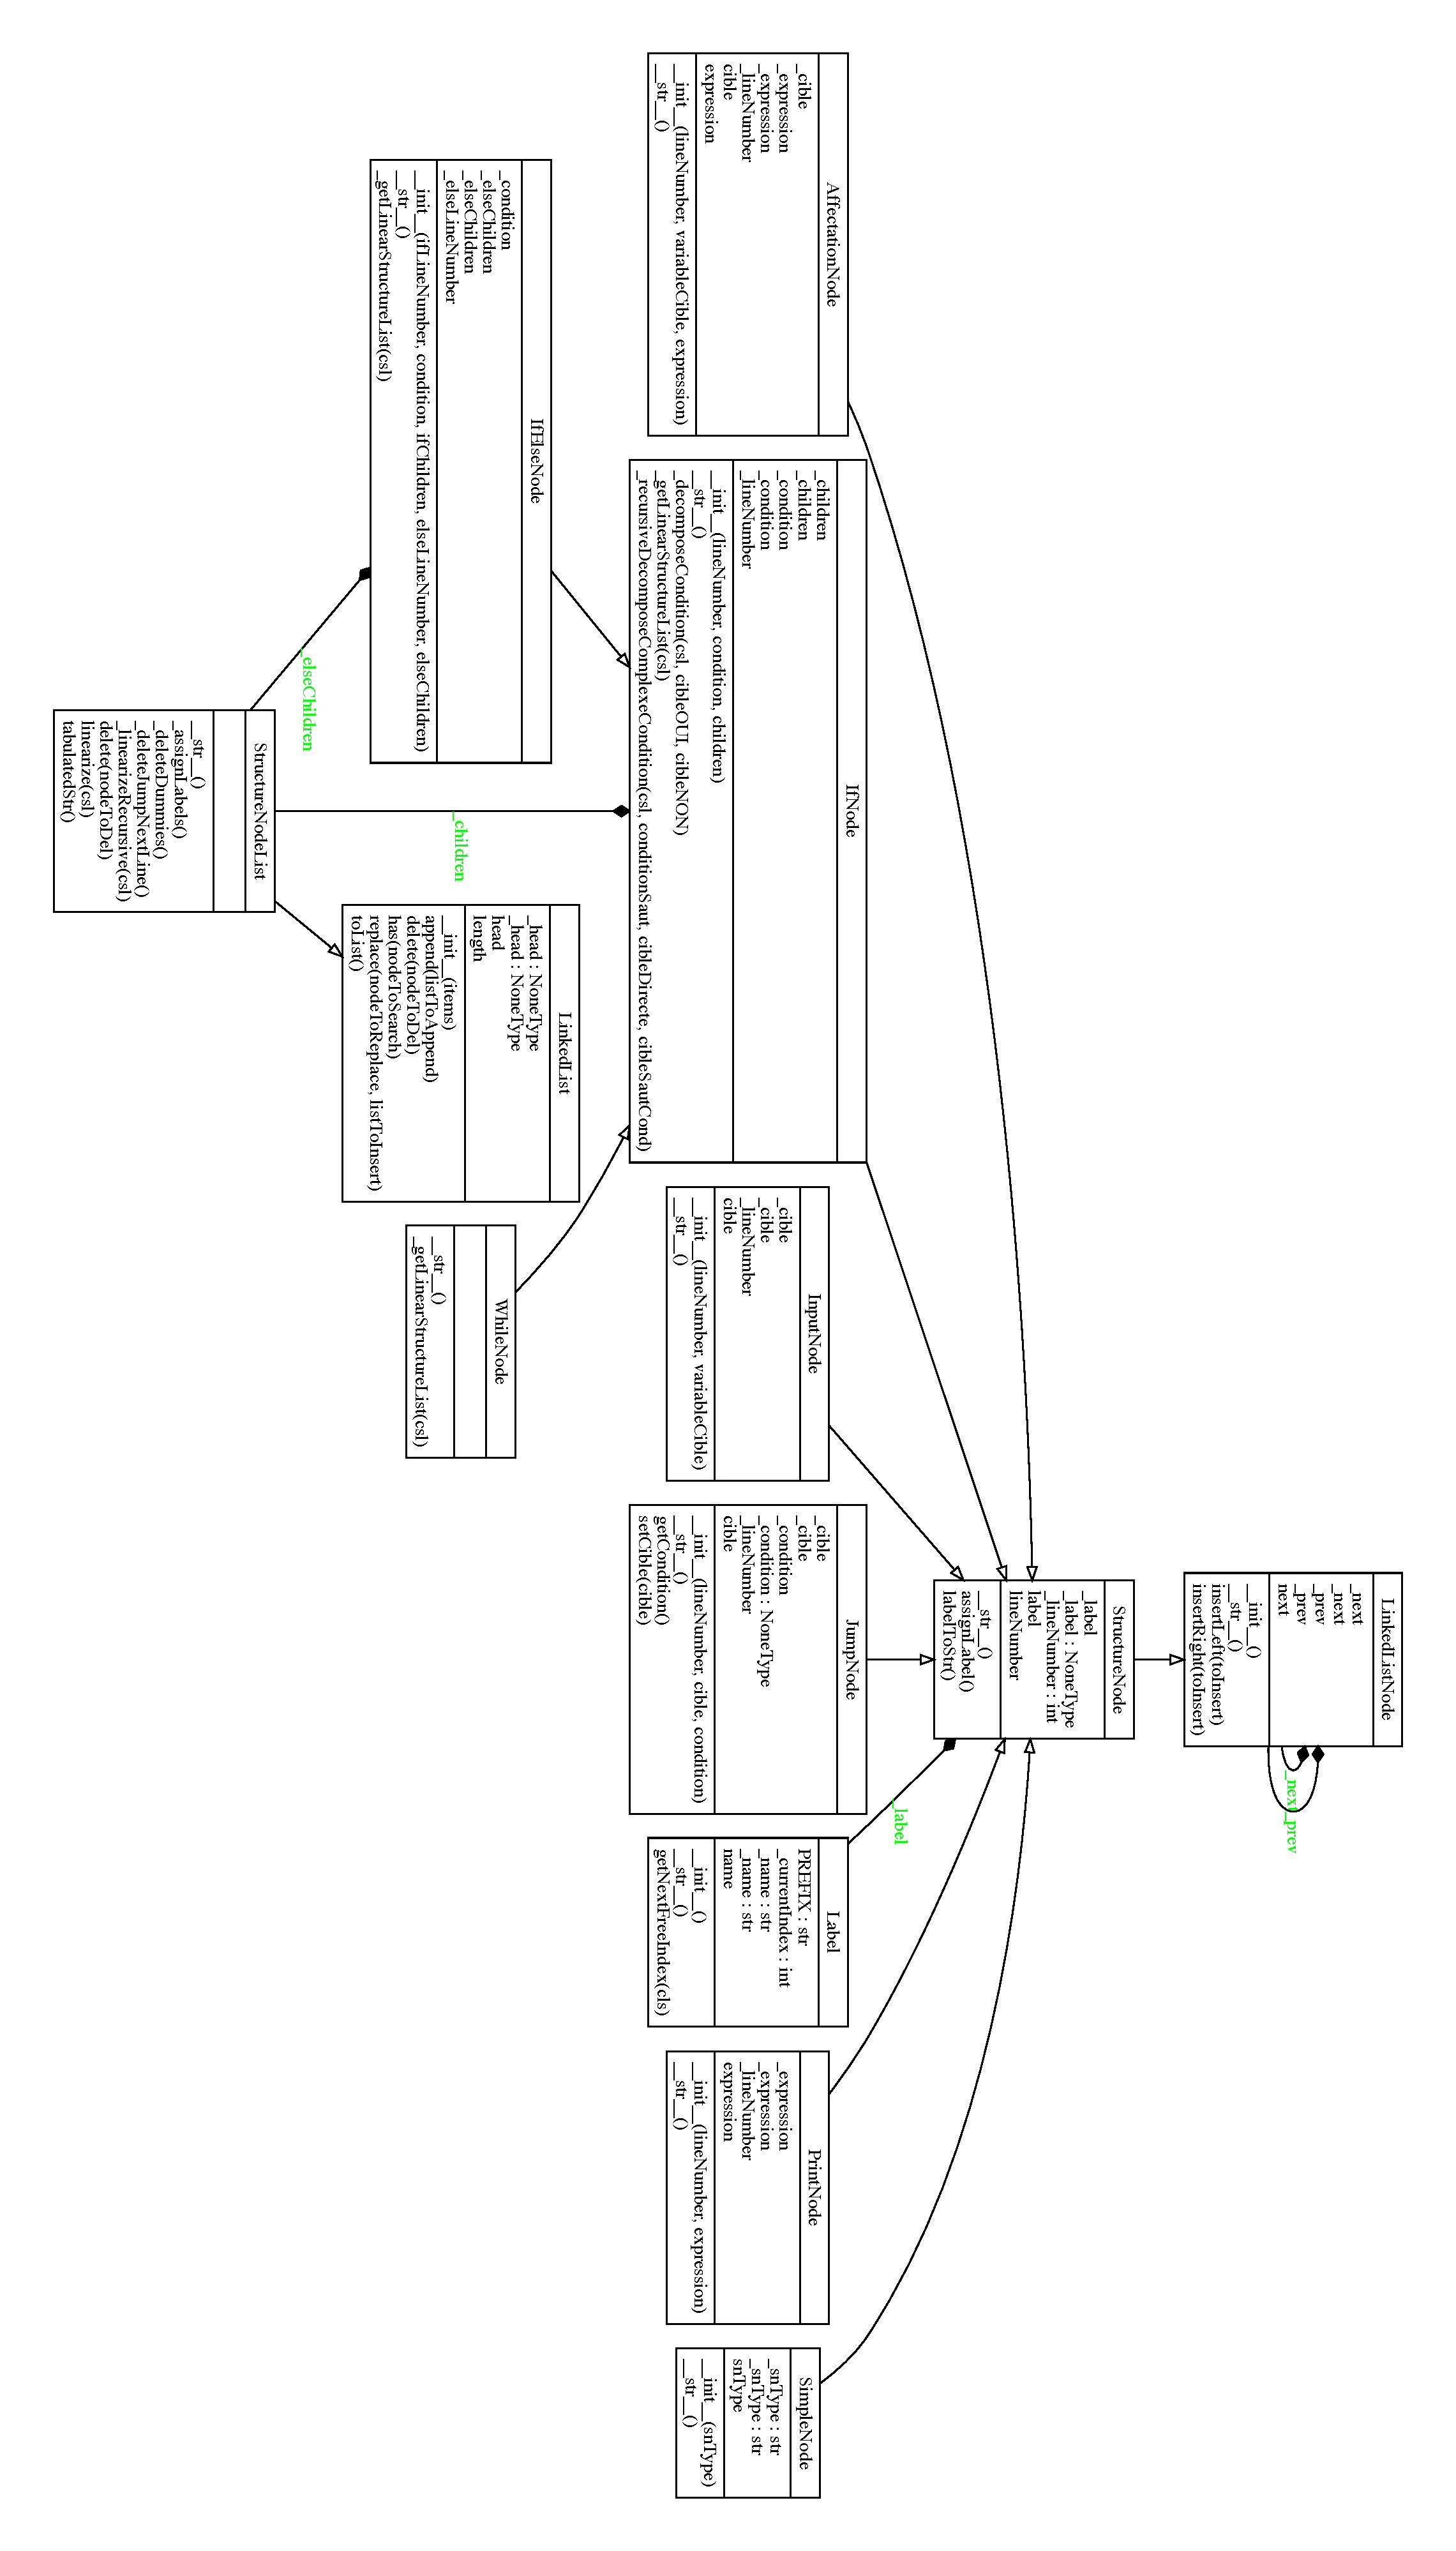
\includegraphics[height=25cm]{./Pictures/StructureNode.pdf}
	\caption{\label{fig:class_StructureNode}Diagramme de classes - StructureNode}
\end{figure}

Les classes héritées de \pyinline{StructureNode} sont présentées sur la figure \ref{fig:class_StructureNode}. On remarquera que les \pyinline{StructureNode} peuvent être des structures de données récursives, les n\oe uds de type \pyinline{IfNode}, \pyinline{IfElseNode} et \pyinline{WhileNode} ayant pour attribut \pyinline{_children} de type \pyinline{StructureNodeList}.

La classe \pyinline{StructureNode} est en particulier en charge d'assurer la linéarisation des boucles \pyinline{while} et des branchements \pyinline{if} en une série de sauts conditionnels ou inconditionnels
avec la méthode \pyinline{getLinearStructureList(csl)} où \pyinline{csl} est une liste de chaine de caractères correspondant aux symboles de comparaison disponibles dans le modèle de processeur retenu (\ref{sec:processeur}). Elle peut faire appelle le cas échéant aux méthodes des classes \pyinline{ComparisonExpressionNode} et \pyinline{LogicExpressionNode} afin d'adapter les expressions logiques en conséquence.

\clearpage

\subsubsection{Classes ArithmeticExpressionNode, LogicExpressionNode et ComparisonExpressionNode}

Les conditions des branchements \pyinline{if else} ou les arrêts de boucle \pyinline{while} sont implémentées comme des attributs (\pyinline{_condition}) de n\oe uds de type \pyinline{IfNode}, \pyinline{IfElseNode} et \pyinline{WhileNode}. Elles sont associées à des instances des classes \pyinline{LogicExpressionNode} ou \pyinline{ComparisonExpressionNode}.

\begin{figure}[h!]
	\centering
	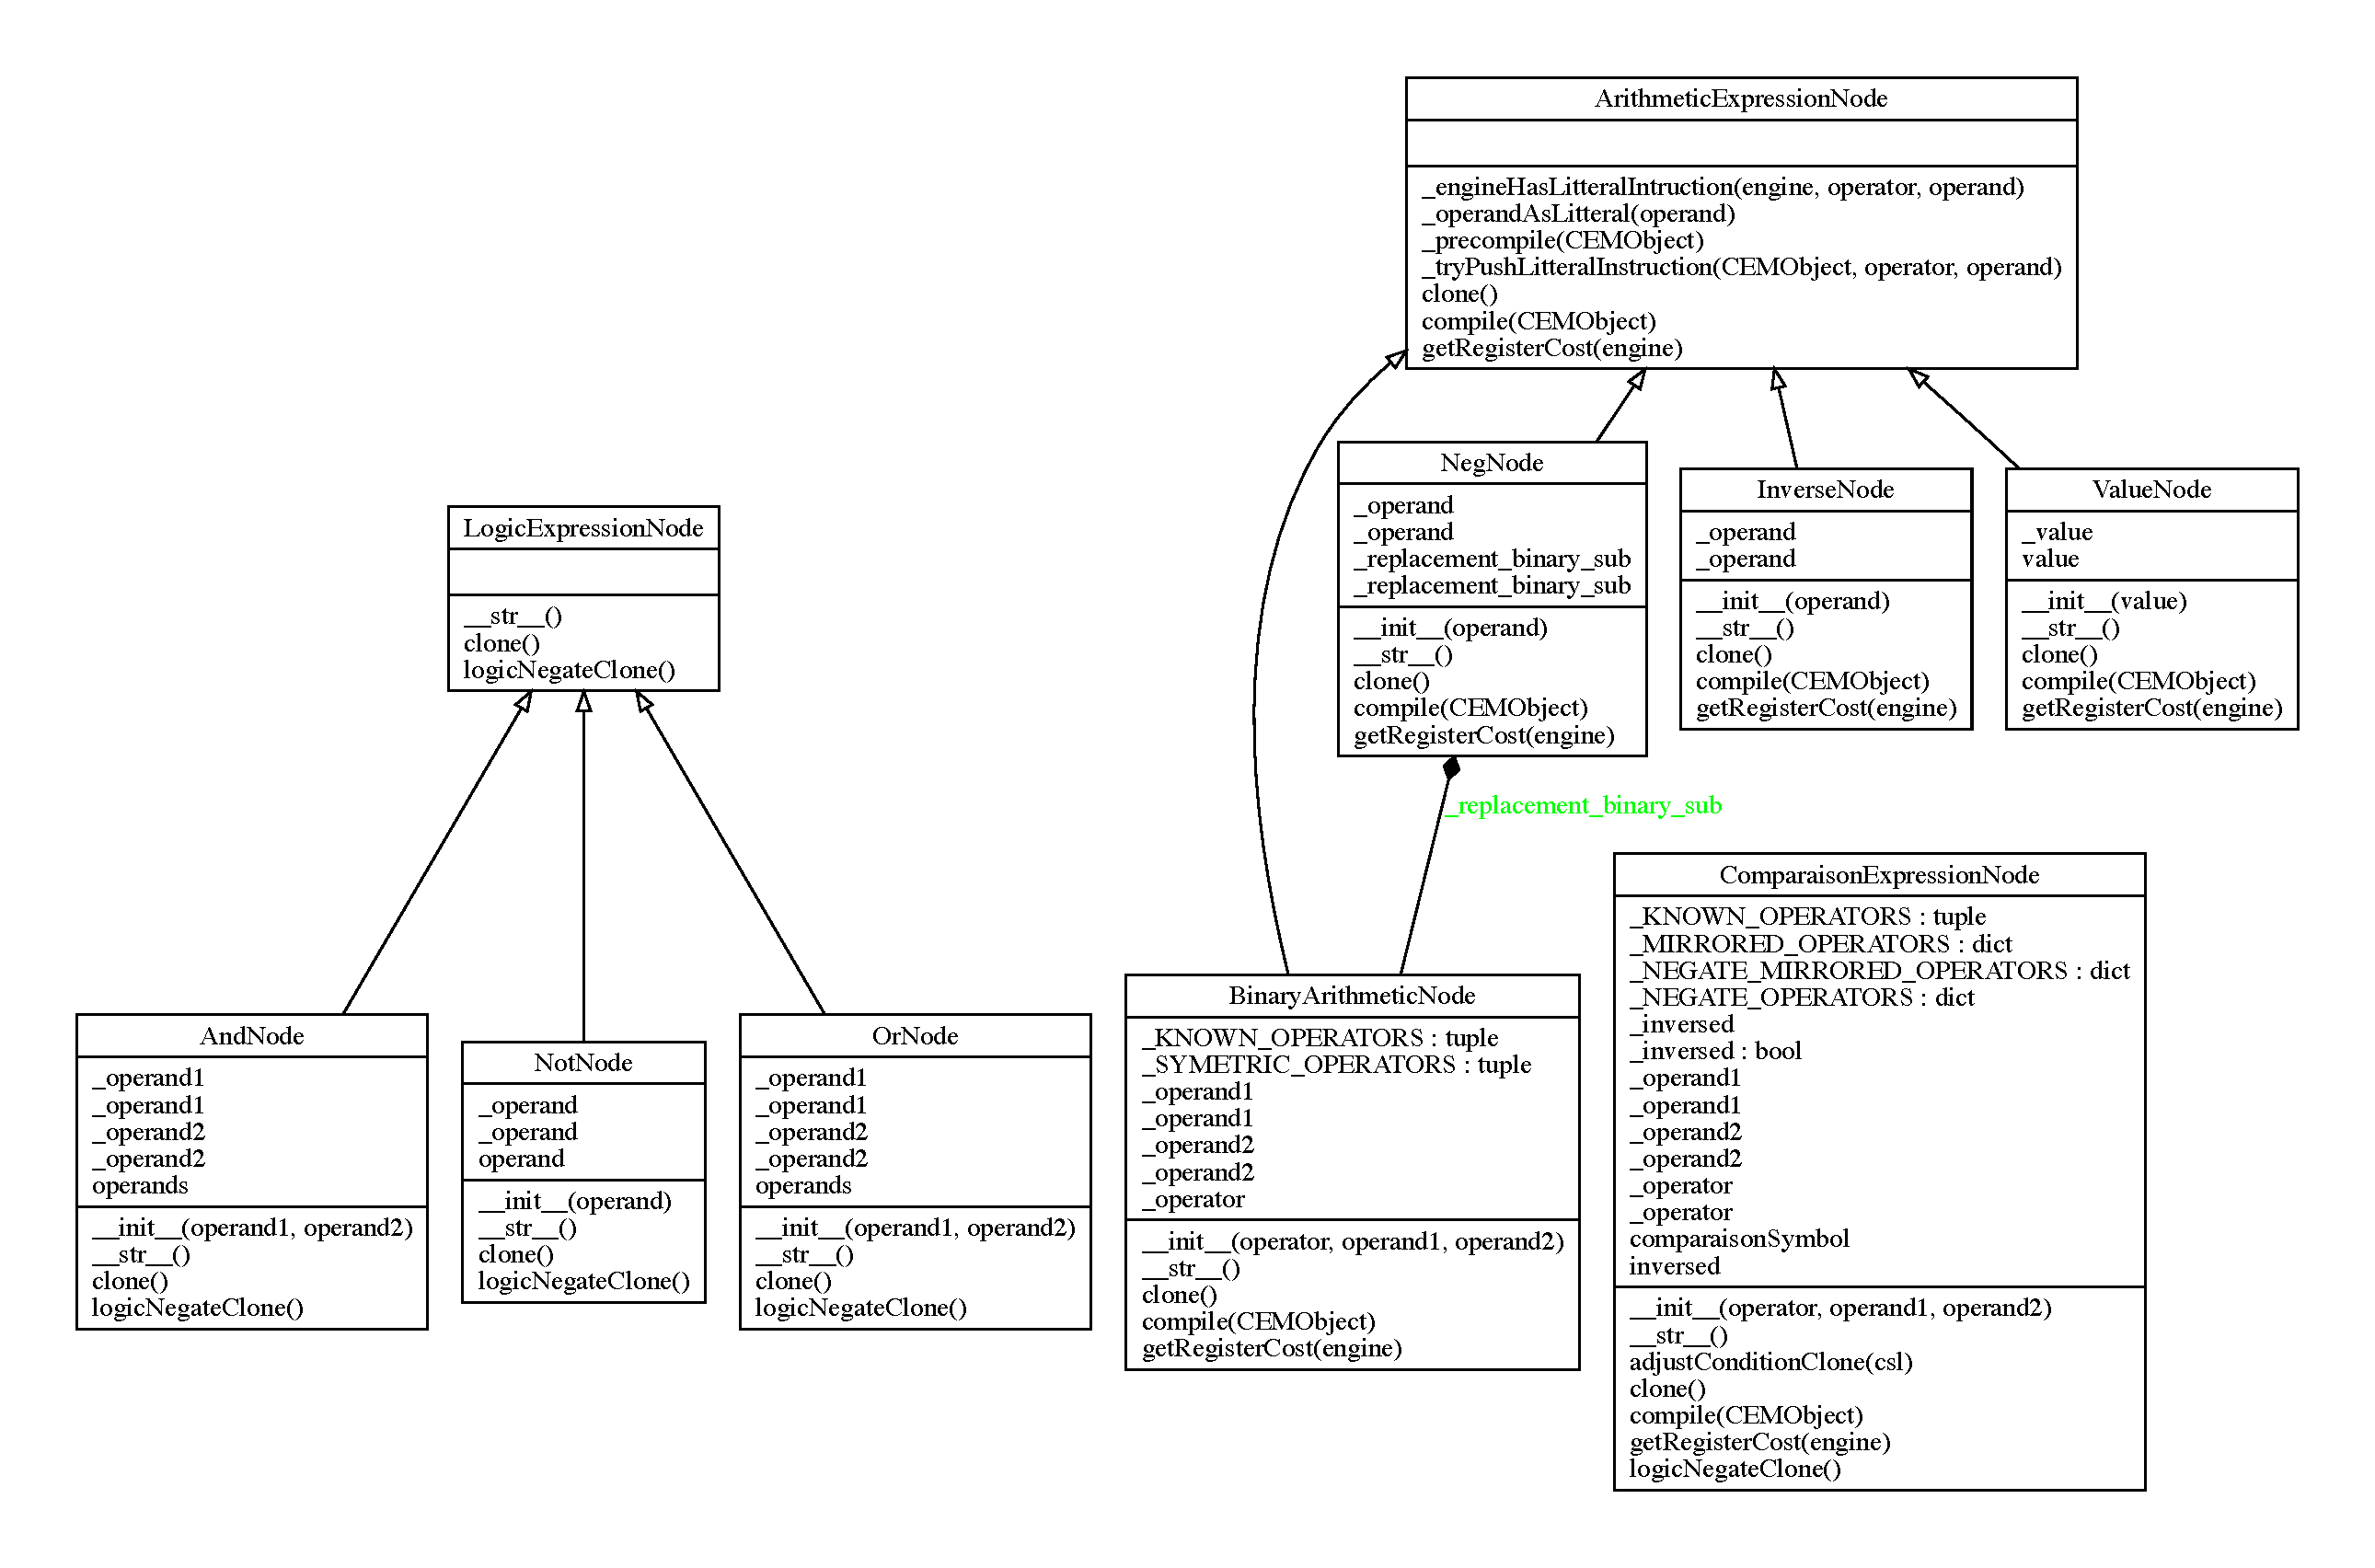
\includegraphics[width=\textwidth]{./Pictures/ExpressionNode.pdf}
	\caption{\label{fig:class_ExpressionNode}Diagramme de classes - ExpressionNode}
\end{figure}

Les expressions de type comparaisons (\pyinline{ComparisonExpressionNode}), expressions arithmétiques \pyinline{ArithmeticExpressionNode} ou les affectations (\pyinline{AffectationNode}) peuvent avoir pour attributs des instances de la classe \pyinline{ArithmeticExpressionNode}.


Une série de méthodes a été définie afin de pouvoir adapter l'expression de certaines conditions logiques aux propriétés du processeur (\ref{sec:processeur}). Par exemple, dans le cas où l'unité arithmétique et logique ne permet de tester que le caractère positif d'une valeur, une expression de type \pyinline{e1<e2} sera transformée en \pyinline{0 < e2-e1}. Les méthodes présentées renvoient une copie de l'expression initiale.

\begin{itemize}
	\item Négation logique d'une expression: \pyinline{logicNegateClone()}
	\item Adaptation des conditions: \pyinline{adjustConditionClone(csl)} avec \pyinline{csl} une liste de chaine de caractères correspondant aux symboles de comparaisons disponibles.

	\item \pyinline{negToSubClone()} transforme une expression de la forme \pyinline{-e} en \pyinline{0-e}.  
\end{itemize}
\begin{figure}[h!]
	\centering
	\begin{tikzpicture}
\begin{scope}
	\node[draw, minimum height=1.5em] (begin) at (0,0) {
		\texttt{\#4 > @x}
	};
	
	
	\node[right = 6cm of begin.east, draw, minimum height=1.5em] (end) {
		\texttt{@x < \#4}
	};
	
	\draw[->] (begin.east) -- (end) node[midway, above] {\pyinline{adjustConditionClone(['<', '=='])}};
\end{scope}

\begin{scope}[shift={(0,-1)}]
	\node[draw, minimum height=1.5em] (begin) at (0,0) {
		\texttt{\#8 >= @y}
	};
	
	
	\node[right = 6cm of begin.east, draw, minimum height=1.5em] (end) {
		\texttt{not (\#8 < @y)}
	};
	
	\draw[->] (begin.east) -- (end) node[midway, above] {\pyinline{adjustConditionClone(['<', '=='])}};
\end{scope}
	\end{tikzpicture}
	
	\caption{adjustConditionClone: exemples. Seuls les opérateurs \pyinline{<} et \pyinline{==} sont disponibles dans le modèle de processeur}
\end{figure}

\clearpage
\subsection{Compilation}
L'étape de compilation doit permettre de transcrire la liste linéarisée de \pyinline{StructureNode} obtenue à l'issue de la phase d'analyse (\cref{sec:ParsedCode}) dans le code assembleur et le code binaire correspondant au modèle de processeur retenu (\cref{sec:processeur}).

\subsubsection{Classe CompilationManager}

La compilation est assurée par une instance de la classe \pyinline{CompilationManager}. Le code assembleur, le binaire et les méthodes associées sont gérés par une instance de la classe \pyinline{AssembleurContainer}.

Pour chaque \pyinline{StructureNode}, \pyinline{CompilationManager.__pushNodeAsm} détermine le type de n\oe ud et délègue à l'instance \pyinline{AssembleurContainer} la création du code assembleur et binaire correspondant.

Lorsque le n\oe ud nécessite l'évaluation d'une expression arithmétique ou d'une comparaison, la compilation est gérée par une instance de la classe \pyinline{CompileExpressionManager}

\begin{figure}[h!]
	\vspace{-1cm}
	\centering
	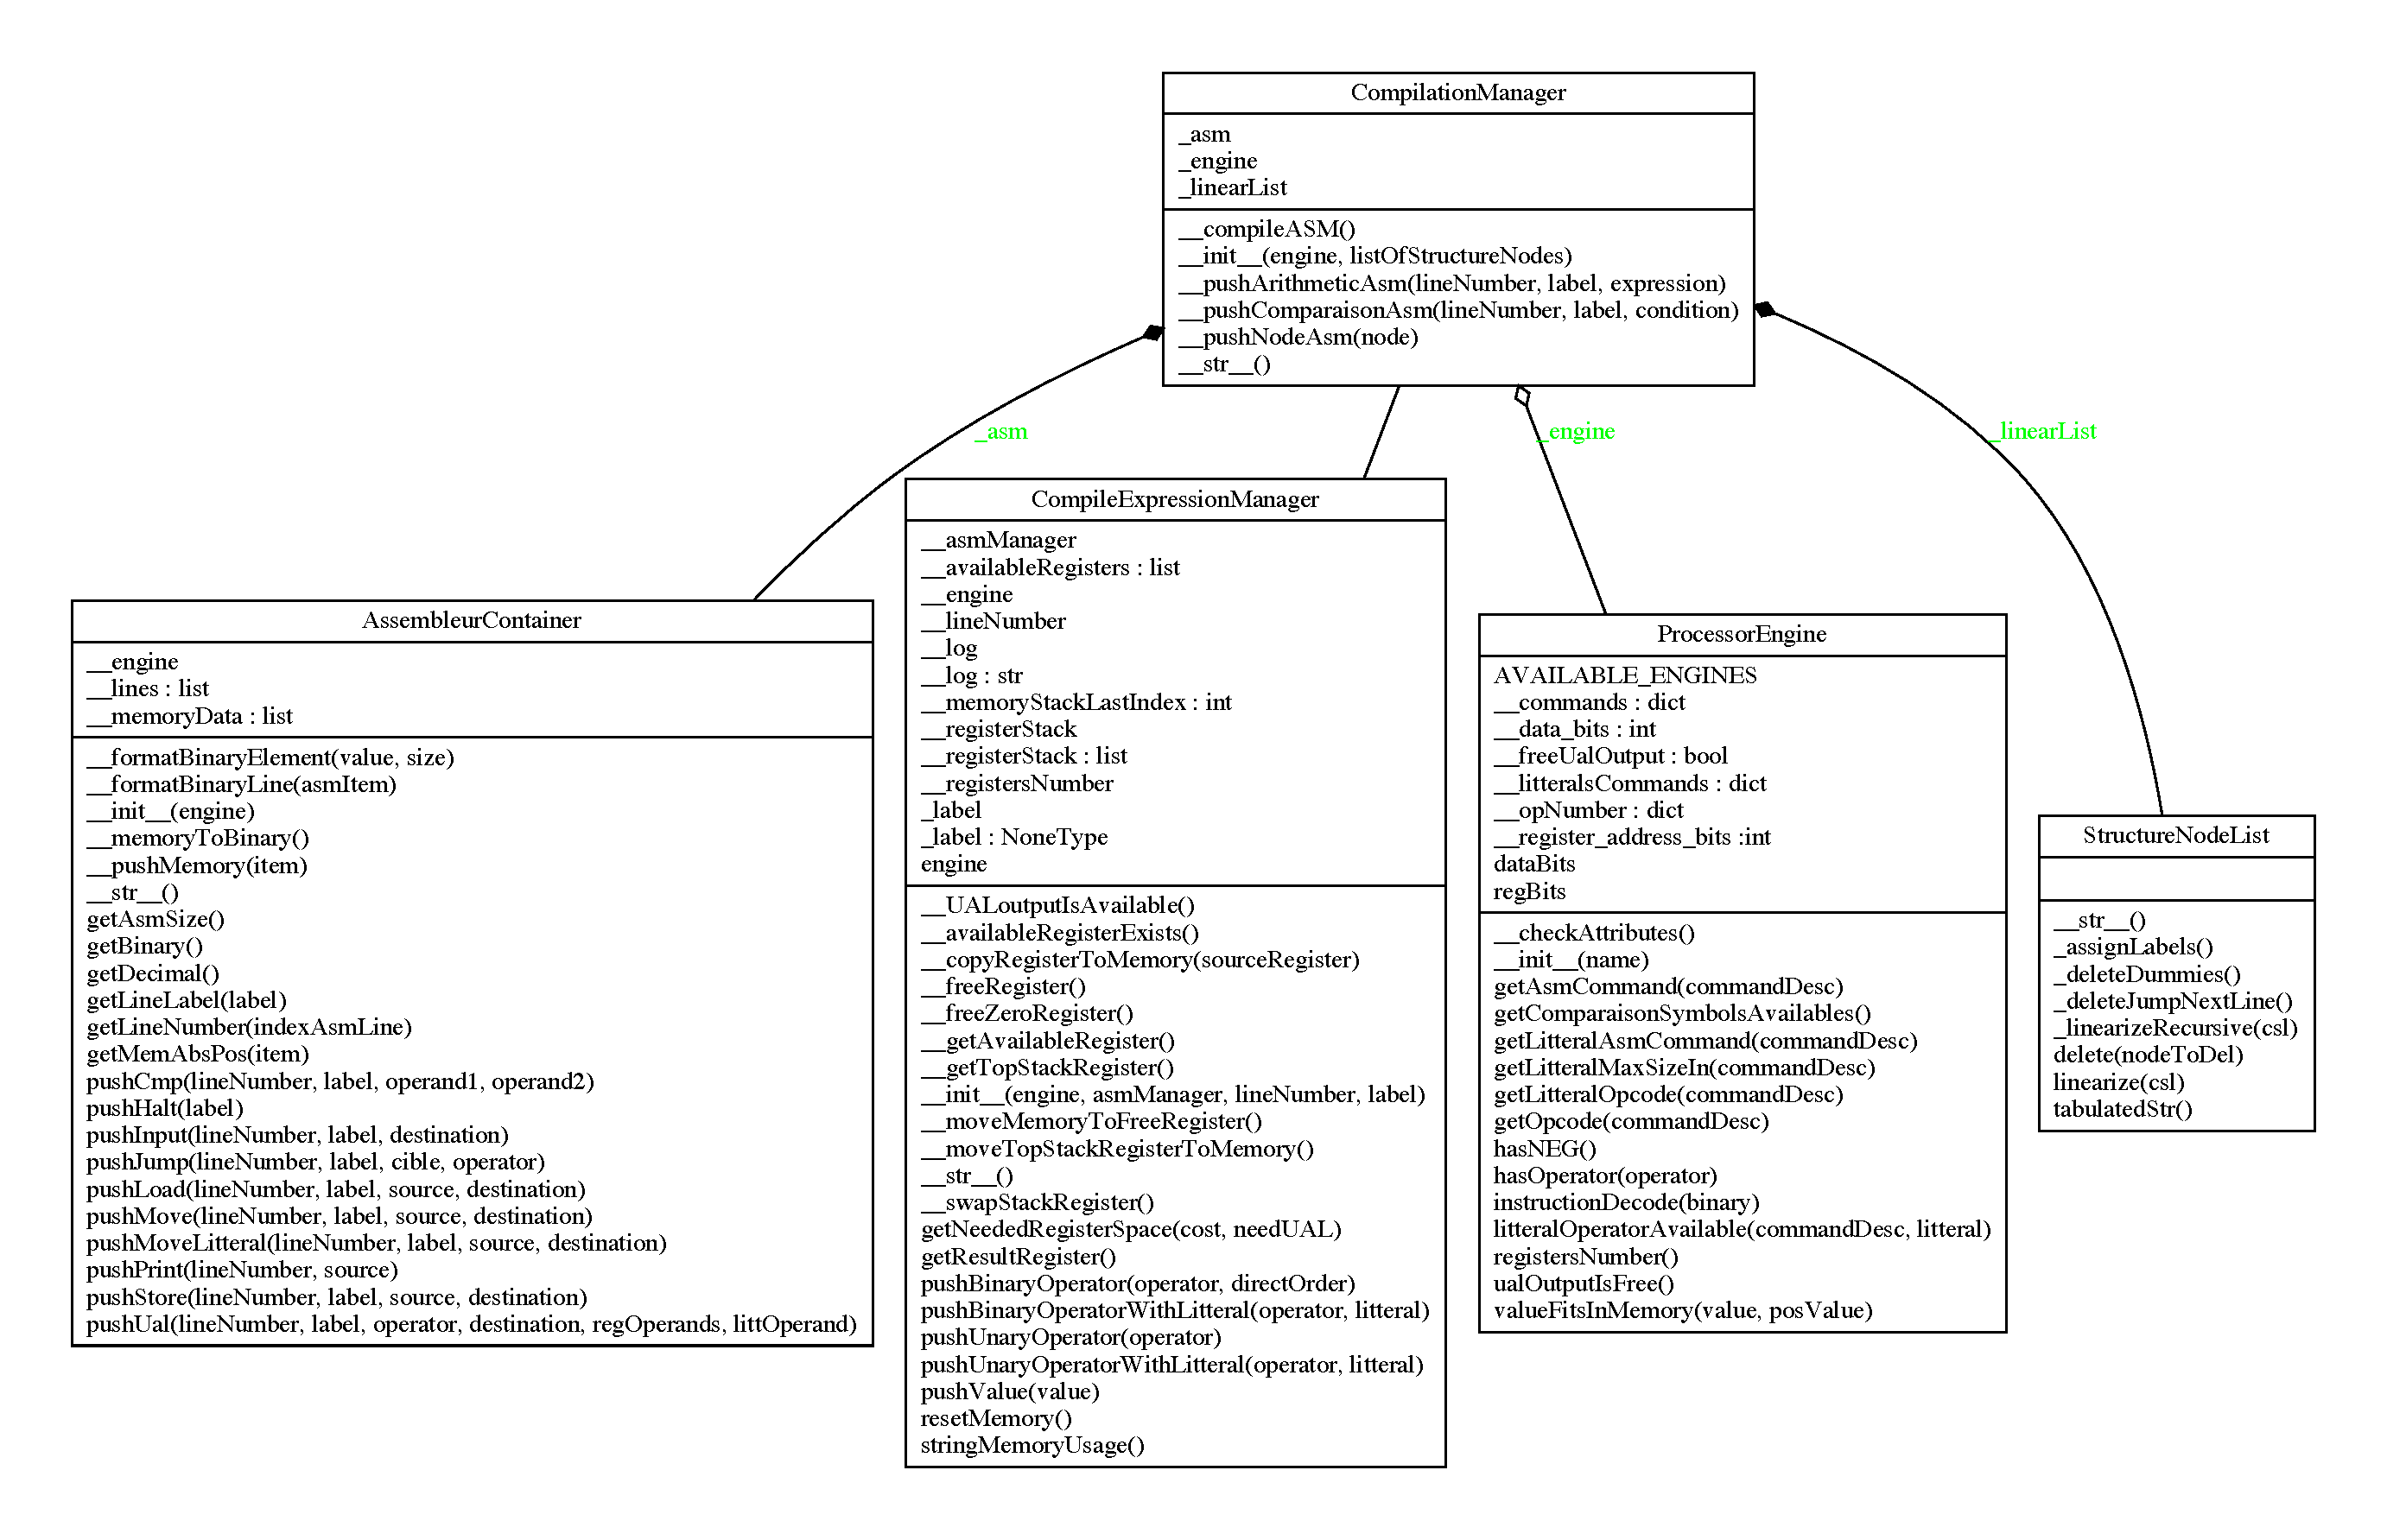
\includegraphics[width=\textwidth]{./Pictures/CompilationManager.pdf}
	\caption{\label{fig:class_CompileManager}Diagramme de classes - Compilation}
\end{figure}

\subsubsection{CompileExpressionManager}
\pyinline{CompilationManager} délègue à la classe\pyinline{CompileExpressionManager} la production du code assembleur liée aux expressions arithmétiques et aux comparaisons. En particulier tout ce qui concerne:
\begin{itemize}
	\item la gestion des registres et pile de registre,
	\item la gestion de mémoire et pile mémoire,
	\item les transferts entre registres et mémoire.
\end{itemize}


\subsubsection{AssembleurContainer}
\pyinline{AssembleurContainer} a en charge l'ensemble des opérations liées à la manipulation aux codes assembleur et binaire (transtypage, conversion) ainsi que la responsabilité de la production du code pour les objets de type \pyinline{StructureNode}.


\clearpage
\subsection{\label{sec:interface}Interface utilisateur}
L'interface utilisateur a été implémenté à l'aide de la bibliothèque graphique Tkinter. Elle dispose de deux modules:
\begin{enumerate}
	\item un module d'édition du code jouet permettant le chargement, l'édition et l'enregistrement de scripts
	\item un module d'exécution disponible après compilation permettant:
	\begin{itemize}
		\item l'affichage du code assembleur et du binaire associé;
		\item le suivi des registres, mémoire et pointeurs associés;
		\item le suivi des appels UAL;
		\item une sortie et une entrée.
	\end{itemize}
\end{enumerate}
Les deux modules disposent par ailleurs d'un affichage permettant de commenter l'exécution en cours.

\begin{figure}[h!]
	\centering
	\begin{subfigure}{\textwidth}
		\centering
		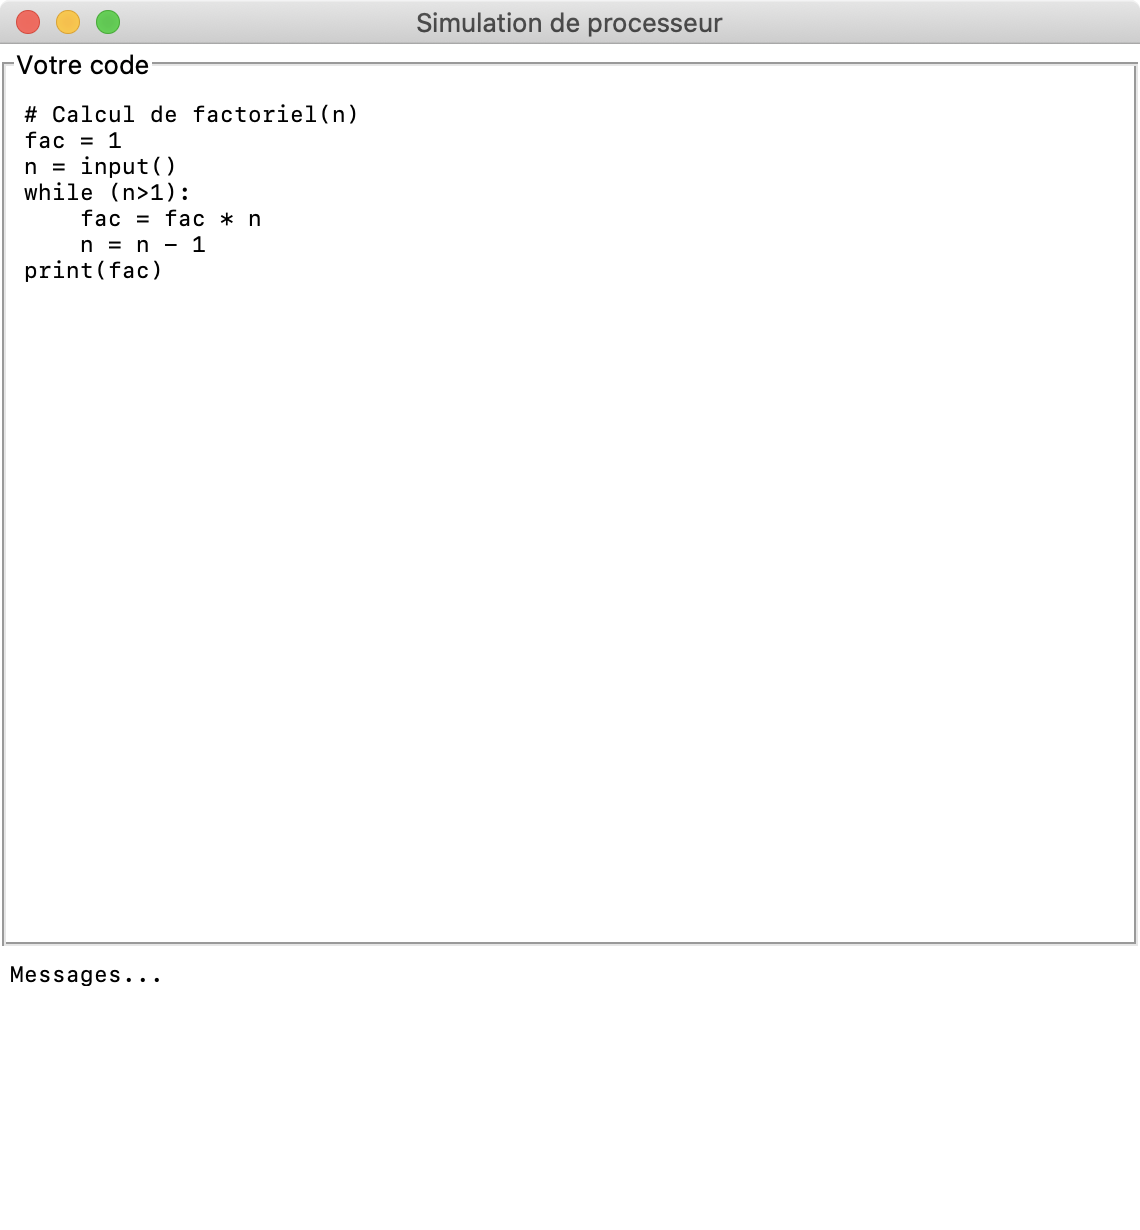
\includegraphics[height=8cm]{./Pictures/EditGUI.png}
		\caption{Module Édition}
	\end{subfigure}
	\begin{subfigure}{\textwidth}
		\centering
	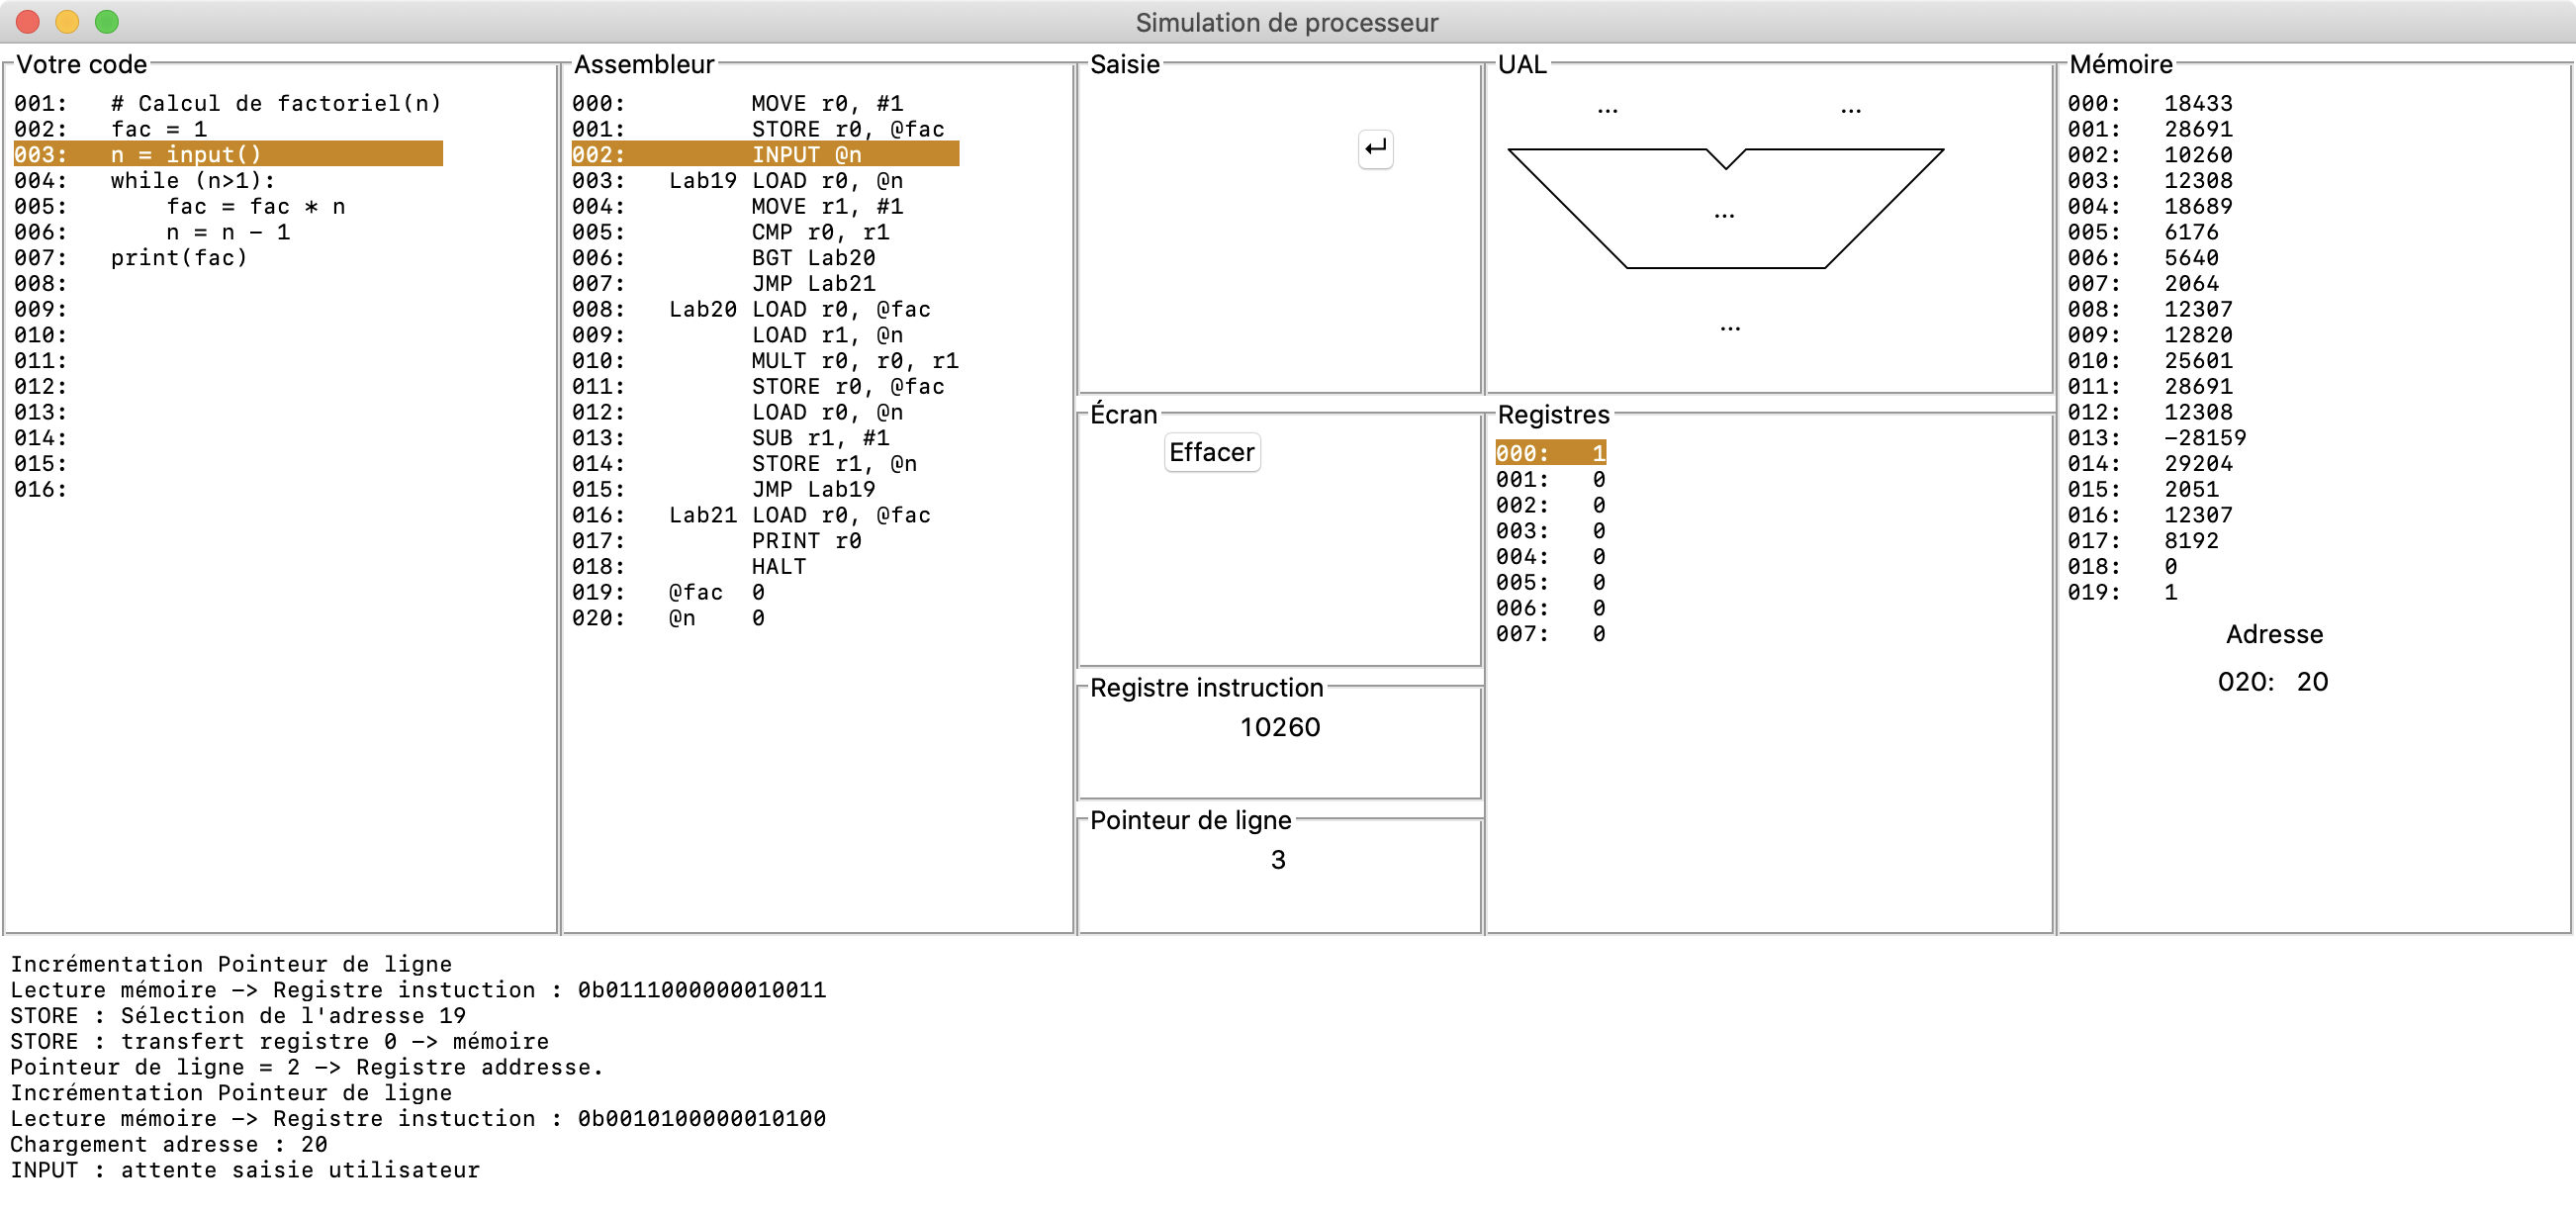
\includegraphics[height=8cm]{./Pictures/ExecGUI.png}
	\caption{Module Exécution}
\end{subfigure}
\caption{Interface graphique}
\end{figure}

\clearpage
\subsection{Gestion de la documentation}
La gestion de la documentation a initialement été mise en place sous la forme d'un wiki sur le dépôt github du projet: \href{https://github.com/gromax/uPSimulator/wiki}{uPSimulator: Simulateur de processeur} (\url{https://github.com/gromax/uPSimulator/wiki})

Dans un second temps, le choix s'est porté sur \href{https://www.sphinx-doc.org/en/master/index.html}{Sphinx} qui permet de renseigner directement le code source, d'exporter dans de multiples formats et d'inclure des fragments exemples.



\clearpage
\section{Organisation}
\subsection{Outils de suivi}
\paragraph{Gestion de projet}

Le suivi de gestion de projet a été réalisé sur l'instance Redmine installée par Pascal Padilla sur un serveur de l'IREM (\url{https://pp.irem.univ-mrs.fr/projects/ctes-projet-mathematiques-informatique/}). Cet outil aura été mis à profit pour assurer le suivi des demandes et la planification, et se sera révélé aussi bien adapté pour centraliser et garder trace des échanges (forum).

\paragraph{Gestion de version}
La gestion de version a été réalisée sur Github (\url{https://github.com/gromax/uPSimulator})

\subsection{Planification}
L'organisation des tâches et le planning associé sont présentés sur la \cref{fig:Gantt}.
\begin{figure}[h!]
	\centering
	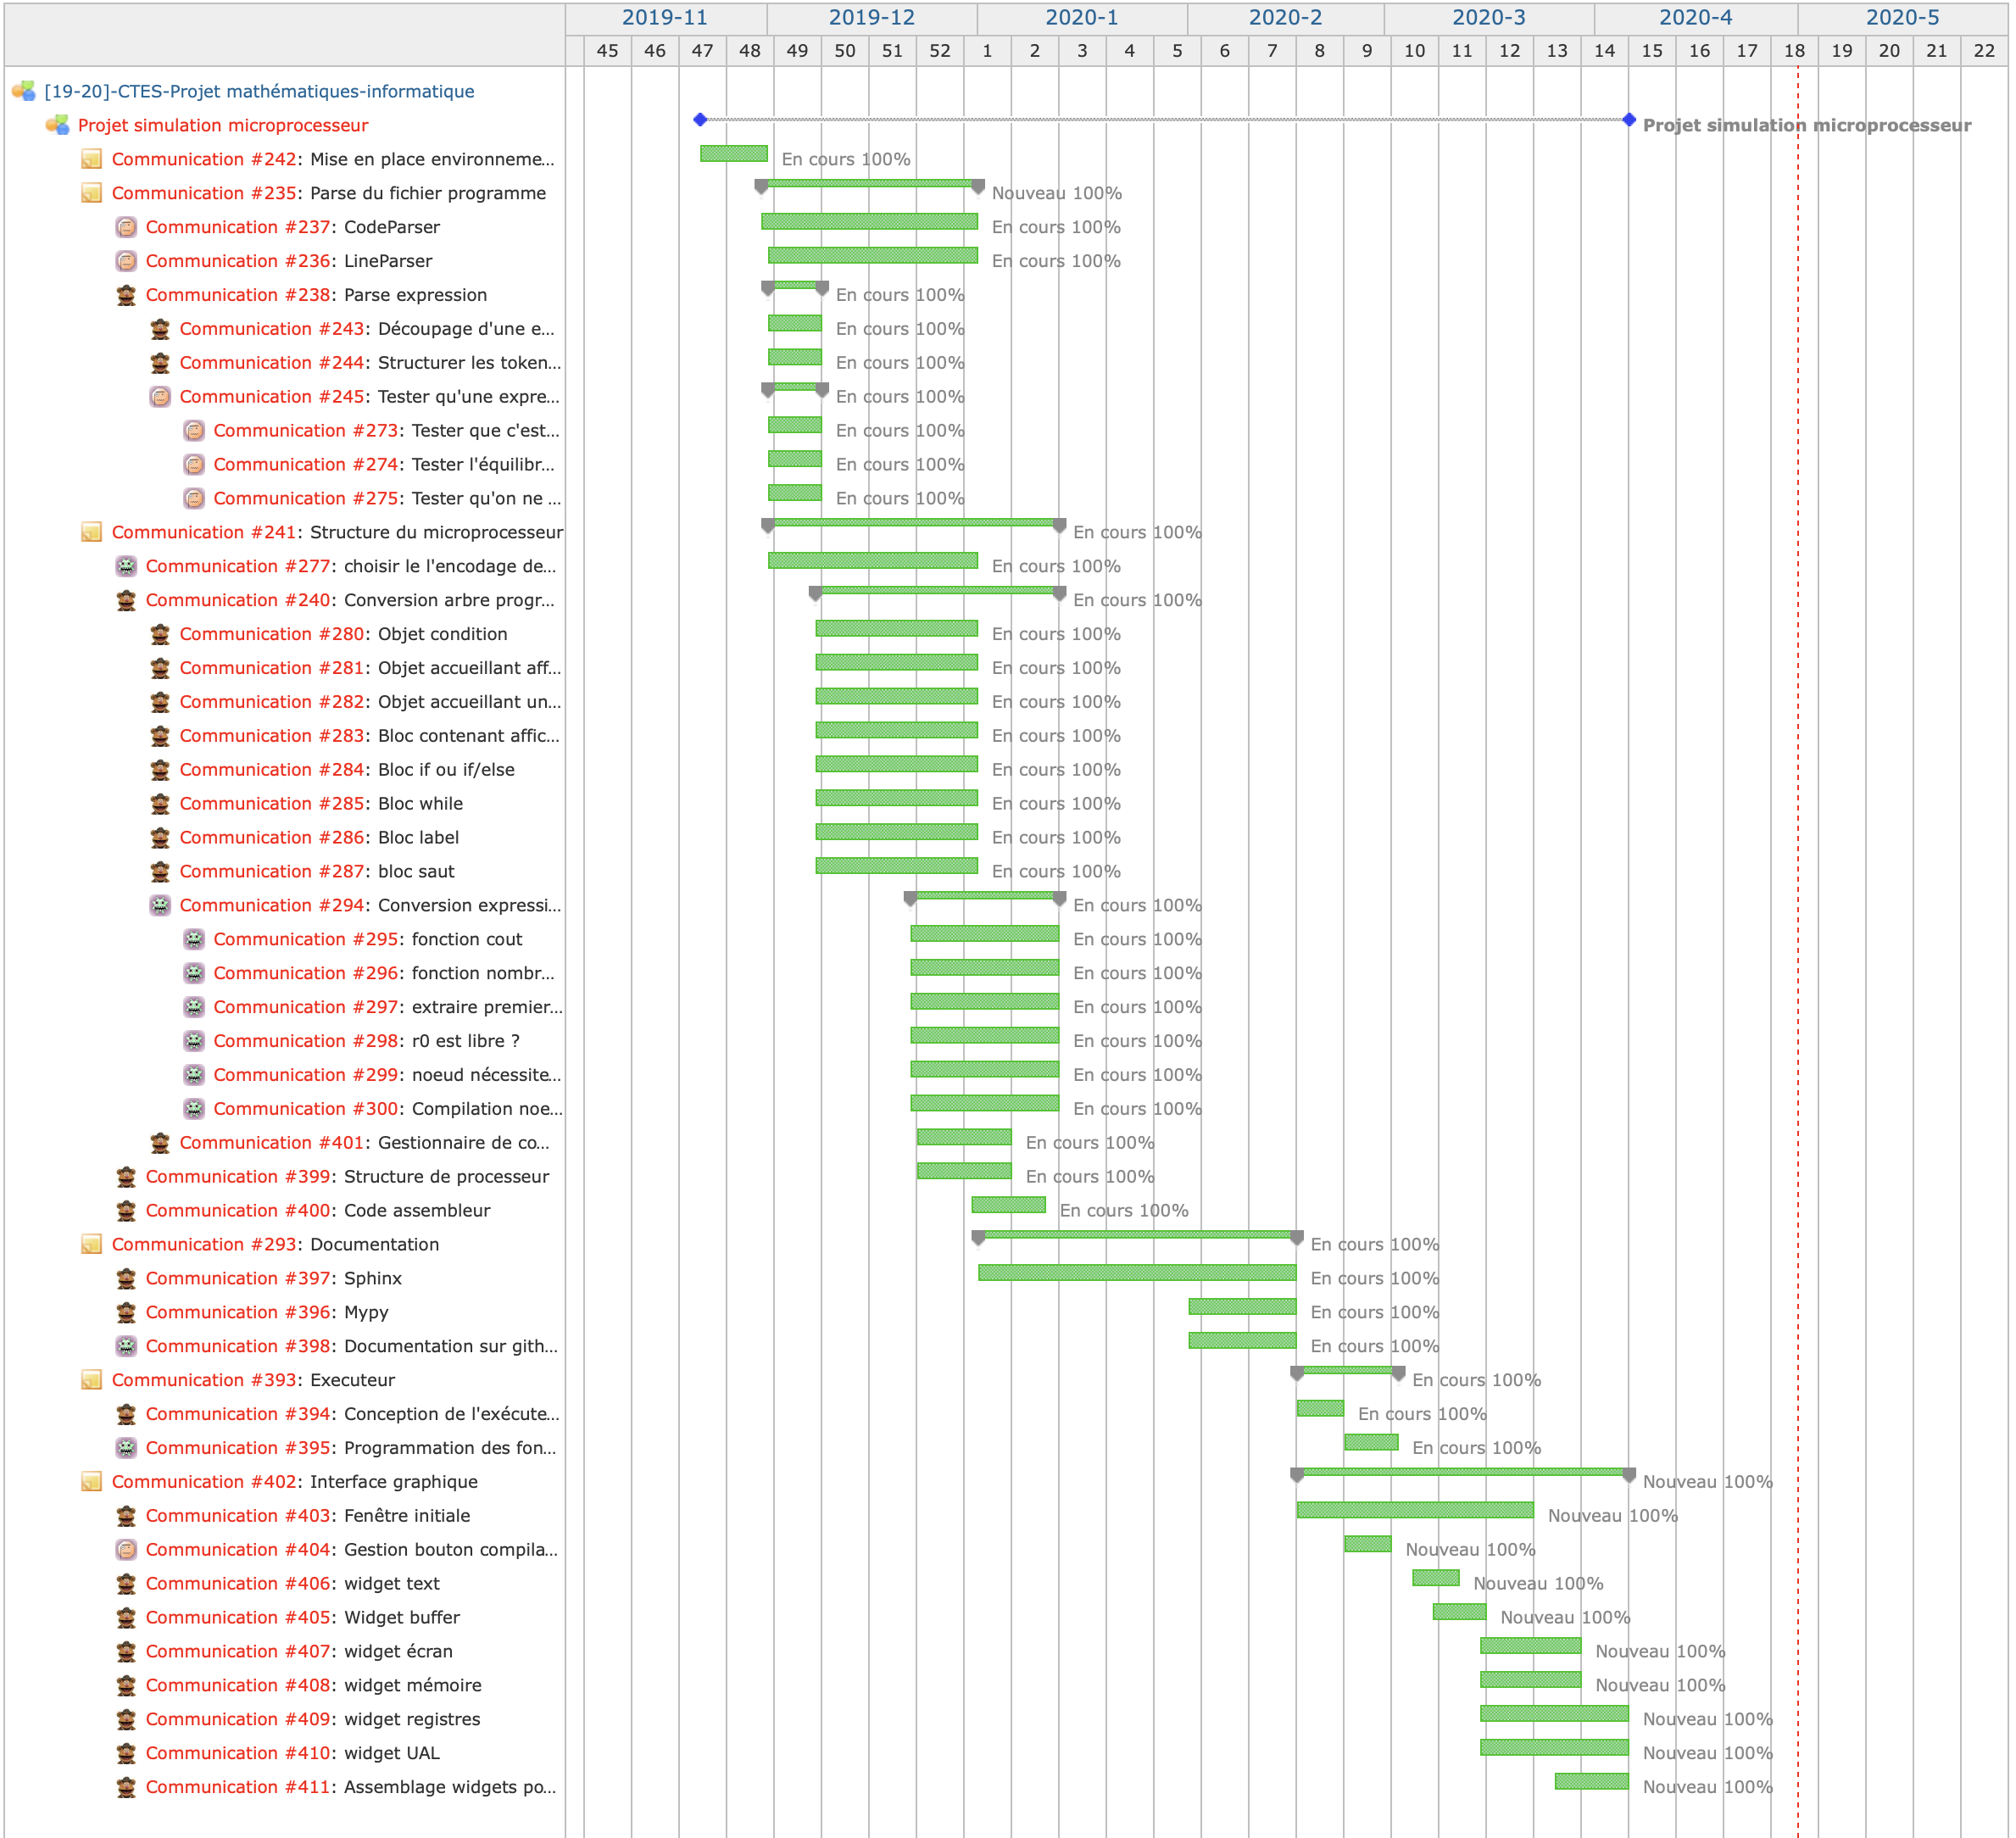
\includegraphics[width=0.9\textwidth]{./Pictures/Gantt.png}
	\caption{\label{fig:Gantt}Diagramme de Gantt du projet}
\end{figure}

\subsection{Répartition des tâches}

Le projet a été imaginé et conçu par Maxence Klein. La connaissance fine de l'objet physique modélisé, des contraintes pédagogiques attendues mais aussi des concepts de programmations à mettre en \oe uvre ont très rapidement mis en lumière un différentiel de compétences important avec les autres membres du projet . Il a dès le départ assumé pleinement son rôle de chef de projet en organisant le travail, en détaillant les taches à réaliser et les solutions techniques à implémenter. 

Véronique Reynaud et Guillaume Desjouis ont pu assurer la mise en \oe uvre de certains éléments techniques sur la base du cahier des charges détaillé établi tandis que l'intégration finale était assuré par Maxence.

\begin{appendix}
\listoffigures
\begingroup
\let\clearpage\relax
\listoftables
\endgroup
\end{appendix}

\end{document}